%Dokumentinformationen
\newcommand{\titleinfo}{Ph2HAT - Formelsammlung}
\newcommand{\authorinfo}{S. Roth, F. Söllner}
\newcommand{\versioninfo}{v1.0 / Juli 2019}
\newcommand{\licence}{CC BY-NC-SA}


%weitere Autoren: ==========================================================================
% S. Roth, F. Söllner

% standard header
%Schriftgr"osse, Layout, Papierformat, Art des Dokumentes
\documentclass[10pt,twoside,a4paper,fleqn]{article}
%Einstellungen der Seitenr"ander
\usepackage[left=1cm,right=1cm,top=1cm,bottom=1cm,includeheadfoot]{geometry}
% Sprache, Zeichensatz, packages
\usepackage[utf8]{inputenc}
\usepackage[ngerman]{babel,varioref}
\usepackage{amssymb,amsmath,fancybox,graphicx,color,colortbl,lastpage,wrapfig,fancyhdr,hyperref,verbatim, mathtools}
\usepackage{titlesec}
\usepackage{textcomp}

\setcounter{secnumdepth}{4}

%pdf info
\hypersetup{pdfauthor={\authorinfo},pdftitle={\titleinfo},colorlinks=false}
%linkbordercolor=white
\author{\authorinfo}
\title{\titleinfo}

%Kopf- und Fusszeile
\pagestyle{fancy}
\fancyhf{}
%Linien oben und unten
\renewcommand{\headrulewidth}{0.5pt} 
\renewcommand{\footrulewidth}{0.5pt}

\fancyhead[L]{\titleinfo{ }\tiny{(\versioninfo)}}
%Kopfzeile rechts bzw. aussen
\fancyhead[R]{Seite \thepage { }von \pageref{LastPage}}
%Fusszeile links bzw. innen
\fancyfoot[L]{\footnotesize{\authorinfo}}
%Fusszeile rechts bzw. ausen
\fancyfoot[R]{\footnotesize{\today}}
%Fusszeile mitte
\fancyfoot[C]{\footnotesize{\licence \quad $\rightarrow$ \href{https://github.com/HSR-Stud}{Github: HSR-Stud}}}



 % ./header.tex nicht editieren (Projekt LaTeX-Header benutzen)

%%%%%%%%%%%%%%%%%%%%%%%%%%%%%%%%%%%%%%%%%%%%%%%%%%%%%%%%%%%%%%%%%%%%%%%%%%%%%%%%%%%%%%%%%%%%%%%%
% Neue Befehle und Definitionen                
%%%%%%%%%%%%%%%%%%%%%%%%%%%%%%%%%%%%%%%%%%%%%%%%%%%%%%%%%%%%%%%%%%%%%%%%%%%%%%%%%%%%%%%%%%%%%%%%
\definecolor{black}{rgb}{0,0,0}
\definecolor{red}{rgb}{1,0,0}
\definecolor{white}{rgb}{1,1,1}
\definecolor{grey}{rgb}{0.8,0.8,0.8}
\definecolor{Gray}{gray}{0.85}
\definecolor{lightgreen}{rgb}{0,1,0}
\definecolor{orange}{rgb}{1,0.549,0}
\definecolor{yellow}{rgb}{0.545,0.271,0.075}
\definecolor{violet}{rgb}{0.372,0.224,0.784}
\newcommand{\scriptBlack}[1]{$_{\textcolor{black}{\mbox{\small{S#1}}}}$}
%\newcommand{\formulary}[1]{$_{\textcolor{red}{\mbox{\small{S. #1}}}}$}
\newcommand{\myparagraph}[1]{\paragraph{#1}\mbox{}\\}

\DeclareMathOperator\arsinh{arsinh}
\DeclareMathOperator\arcosh{arcosh}
\DeclareMathOperator\artanh{artanh}
\DeclareMathOperator\arcoth{arcoth}

\begin{document}
\tableofcontents

%%%%%%%%%%%%%%%%%%%%%%%%%%%%%%%%%%%%%%%%%%%%%%%%%%%%%%%%%%%%%%%%%%%%%%%%%%%%%%%%%%%%%%%%%%%%%%%%
% Hydrostatik                                   
%%%%%%%%%%%%%%%%%%%%%%%%%%%%%%%%%%%%%%%%%%%%%%%%%%%%%%%%%%%%%%%%%%%%%%%%%%%%%%%%%%%%%%%%%%%%%%%%
\newpage
\section{Fluide}
	\subsection{Einführung}
	\subsubsection{Definitionen}
		\begin{minipage}{19cm}
			\begin{itemize}
				\item \textbf{ideale Flüssigkeit:}
					\begin{itemize}
						\item Reibungsfrei (nicht viskos)
						\item Inkompressibel
					\end{itemize}
			\end{itemize}
		\end{minipage}
	\newline
	\newline
	
	\subsubsection{Druck}
		\begin{minipage}[t]{13cm}
			\myparagraph{Definition}
				\renewcommand{\arraystretch}{2.5}
				\begin{tabular}{ p{4cm} p{7cm}}
					$p = \dfrac{F_{\perp}}{A}$	&	$p$ = Druck in $\frac{N}{m^2}$ = $Pa$\\
					$\tau = \dfrac{F_{\parallel}}{A} $	& $\tau$ = Schubspannung in $\frac{N}{m^2}$\\
				\end{tabular}
				\renewcommand{\arraystretch}{1.5}
				\begin{tabular}{ p{4cm} p{7cm} }
					& $F_{\perp}$ = senkrechte Kraftkomponente in $N$\\
					& $F_{\parallel}$ = parallele Kraftkomponente in $N$\\
					& $A$ = Fläche in $m^2$\\
				\end{tabular} 
				\renewcommand{\arraystretch}{1}
		\end{minipage}
		\begin{minipage}[t]{5cm}
			\vspace{-\ht\strutbox}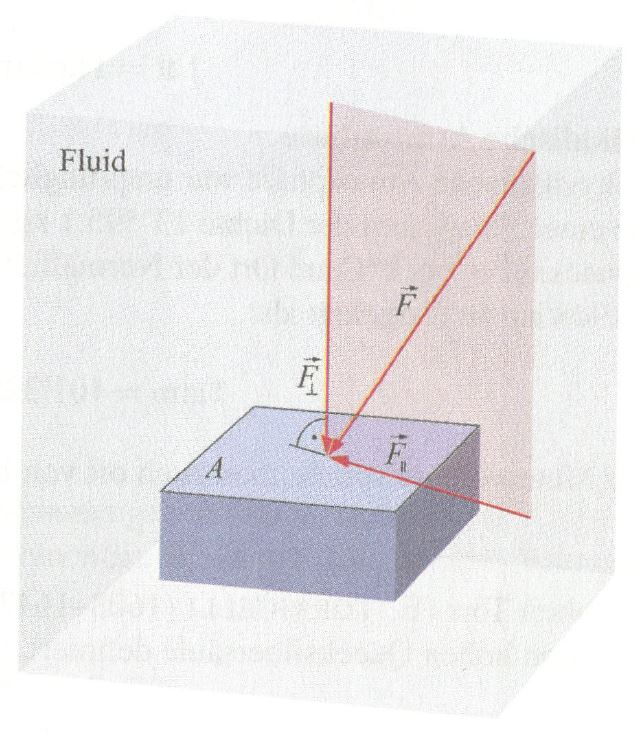
\includegraphics[width=4.5cm]{./bilder/Druck.jpg}
		\end{minipage}
		\newline
		\newline
		\begin{minipage}[t]{12cm}
			\myparagraph{Druckeinheiten}
				\renewcommand{\arraystretch}{1.5}
				\begin{tabular}{ p{4cm} p{9cm}}
					1 bar = $10^5$ Pa\\
					1 at = $9.807 \cdot 10^4$ Pa	&	at = technische Atmosphäre\\
					1 atm = $1.013 \cdot 10^5$ Pa	&	atm = physikalische Atmosphäre\\
					1 Torr = 133.3 Pa	&	Torr = Millimeter Quecksilbersäule\\
					1 psi = $6.895 \cdot 10^3$ Pa	&	psi = angelsächsische Einheit (pound per square inch)\\
				\end{tabular}
				\renewcommand{\arraystretch}{1}
		\end{minipage}
		\newline
		\newline
		\newline
		\newline
		\begin{minipage}[t]{11.5cm}
			\myparagraph{Gesetz von Pascal}
				\newline
				Druck ist nicht Richtungsabhängig!\\ \\
				\renewcommand{\arraystretch}{1.5}
				\begin{tabular}{ p{4cm} p{7cm}}
					$p_a = p_b = p_c$	&	$p_a$ = Druck auf Fläche $a \cdot h$\\
					&	$p_b$ = Druck auf Fläche $b \cdot h$\\
					&	$p_c$ = Druck auf Fläche $c\cdot h$\\
				\end{tabular}\\ \\ \\
		\end{minipage}
		\begin{minipage}[t]{10cm}
			\vspace{-\ht\strutbox}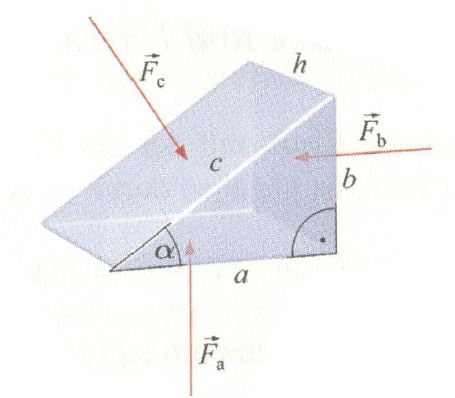
\includegraphics[width=5.5cm]{./bilder/GesetzVonPascal1.jpg}
			\vspace{-\ht\strutbox}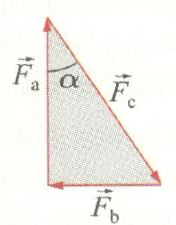
\includegraphics[width=2cm]{./bilder/GesetzVonPascal2.jpg}
		\end{minipage}
	\newpage
	\subsubsection{Kompression}
		\begin{minipage}[t]{13cm}
			\myparagraph{Kompressibilität}
				\renewcommand{\arraystretch}{2.5}
				\begin{tabular}{ p{4cm} p{7cm}}
					$\kappa = -\dfrac{1}{V} \dfrac{\Delta V}{\Delta p}$	&	$\kappa$ = Kompressibilität in $\frac{1}{Pa}$\\
				\end{tabular}
				\renewcommand{\arraystretch}{1.5}
				\begin{tabular}{ p{4cm} p{7cm} }
					& $V$ = Volumen in $m^2$\\
					& $p$ = Druck in $Pa$\\
				\end{tabular} 
				\renewcommand{\arraystretch}{1}
		\end{minipage}
		\newline
		\begin{minipage}[t]{13cm}
			\myparagraph{Kompressionsmodul}
			\renewcommand{\arraystretch}{2.5}
			\begin{tabular}{ p{4cm} p{7cm}}
				$K = \dfrac{1}{\kappa} = -V \dfrac{\Delta p}{\Delta V}$	&	$\kappa$ = Kompressibilität in $\frac{1}{Pa}$\\
			\end{tabular}
			\renewcommand{\arraystretch}{1.5}
			\begin{tabular}{ p{4cm} p{7cm} }
				& $K$ = Kompressionsmodul in $Pa$\\
				& $V$ = Volumen in $m^2$\\
				& $p$ = Druck in $Pa$\\
			\end{tabular} 
			\renewcommand{\arraystretch}{1}
		\end{minipage}

\newpage	
\subsection{Hydrostatik}
	\subsubsection{Schweredruck}
		\begin{minipage}[t]{13cm}
			\myparagraph{Flüssigkeiten}
				\begin{flushleft}
					Hydrostatisches Paradoxon: Der Schweredruck in einer ruhenden Flüssigkeit ist nur von der Höhe in der Flüssigkeit, nicht aber von der Form des Gefässes abhängig.
				\end{flushleft}
				\renewcommand{\arraystretch}{1.5}
				\begin{tabular}{ p{4cm} p{7cm}}
					$p = \rho gh$	&	$p$ = Druck in $Pa$\\
					& $\rho$ = Dichte in $\frac{kg}{m^3}$\\
					& $g$ = Gravitationsfeldstärke = $9.81\frac{m}{s^2}$\\
					& $h$ = Höhe in $m$ (unter Wasseroberfläche)\\
				\end{tabular}
				\renewcommand{\arraystretch}{1}
		\end{minipage}
		\begin{minipage}[t]{10cm}
			\vspace{-\ht\strutbox}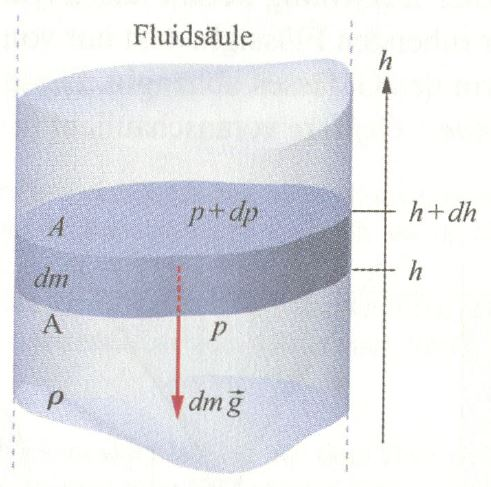
\includegraphics[width=5cm]{./bilder/Schweredruck.jpg}
		\end{minipage}
		\newline
		\newline
		\newline
		\begin{minipage}[t]{13cm}
			\myparagraph{Gase (Barometrische Höhenformel für isotherme Atmosphäre)}
			\renewcommand{\arraystretch}{1.5}
			\begin{tabular}{ p{4cm} p{7cm}}
				$p = p_0 e^{-\frac{\rho_0}{p_0}gh}$	&	$p$ = Druck in $Pa$\\
				& $\rho$ = Dichte in $\frac{kg}{m^3}$\\
				& $g$ = Gravitationsfeldstärke = $9.81\frac{m}{s^2}$\\
				& $h$ = Höhe in $m$\\
			\end{tabular}
			\renewcommand{\arraystretch}{1}
		\end{minipage}
	
	\subsubsection{Statischer Auftrieb (Archimedisches Prinzip)}
		\begin{minipage}[t]{13cm}
			Der Auftrieb eines in ein Fluid eingetauchten Körpers ist gleich dem Gewicht des von ihm verdrängten Fluids.\\
			Der Auftrieb ist unabhängig von der Tiefe!\\ \\
			\renewcommand{\arraystretch}{1.5}
			\begin{tabular}{ p{4cm} p{7cm}}
				$F_A = F_G$	&	$F_A$ = Auftriebskraft in $N$\\
				$F_A = \rho_{fl} \cdot g \cdot V_{fl}$	& $F_G$ = Gewichtskraft in $N$\\
				$F_G = m_K \cdot g = \rho_k \cdot g \cdot V_K$	& $\rho_{fl}$ = Dichte des Fluids in $\frac{kg}{m^3}$\\
				& $\rho_{k}$ = Dichte des Festkörpers in $\frac{kg}{m^3}$\\
				& $V_{fl}$ = Von Festkörper verdrängtes Fluid-Volumen in $m^3$\\
				& $m_K$ = Masse Festkörper in $kg$\\
				& $V_K$ = Volumen Festkörper in $m^3$\\
			\end{tabular}
			\renewcommand{\arraystretch}{1}
		\end{minipage}
		\begin{minipage}[t]{10cm}
			\vspace{-\ht\strutbox}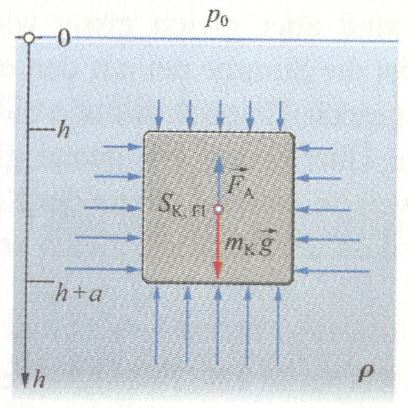
\includegraphics[width=5cm]{./bilder/StatischerAuftrieb.jpg}
		\end{minipage}
	
	\subsubsection{Grenzflächeneffekte}
		\begin{minipage}[t]{10.5cm}
			\myparagraph{Oberflächenspannung, spez. Oberflächenenergie (Van der Waals-Kraft)}
			\newline
			Kräfte zwischen Atomen oder Molekülen an der Oberfläche eines Fluides.\\ \\
			\renewcommand{\arraystretch}{2.5}
			\begin{tabular}{ p{4cm} p{7cm}}
				$\sigma = \dfrac{F}{l} = \dfrac{\Delta W}{\Delta A}$	&	$\sigma$ = Oberflächenspannung in $\frac{N}{m}$\\
			\end{tabular}
			\renewcommand{\arraystretch}{1.5}
			\begin{tabular}{ p{4cm} p{7cm}}
				& \\
				& \\
			\end{tabular}
			\renewcommand{\arraystretch}{1}
		\end{minipage}
		\begin{minipage}[t]{10cm}
			\vspace{-\ht\strutbox}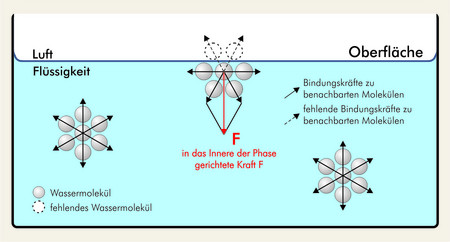
\includegraphics[width=8cm]{./bilder/VanDerWaalsKraft.jpg}
		\end{minipage}
		\newline
		\newline
		\newline
		\begin{minipage}[t]{12cm}
			\myparagraph{Grenzflächenspannung}
			\renewcommand{\arraystretch}{2.5}
			\begin{tabular}{ p{4cm} p{7cm}}
				$cos(\varphi) = \dfrac{\sigma_{sg}-\sigma_{sl}}{\sigma_{lg}}$	&	$\varphi$ = Kontaktwinkel in rad\\
			\end{tabular}
			\renewcommand{\arraystretch}{1.5}
			\begin{tabular}{ p{4cm} p{7cm}}
				& $\sigma_{sl}$ = Grenzflächenspannung zw. Festkörper und Flüssigkeit in $\frac{N}{m}$\\
				& $\sigma_{sg}$ = Grenzflächenspannung zw. Festkörper und Gas in $\frac{N}{m}$\\
				& $\sigma_{lg}$ = Grenzflächenspannung zw. Flüssigkeit und Gas in $\frac{N}{m}$\\
			\end{tabular}
			\renewcommand{\arraystretch}{1}
		\end{minipage}
		\begin{minipage}[t]{10cm}
			\vspace{-\ht\strutbox}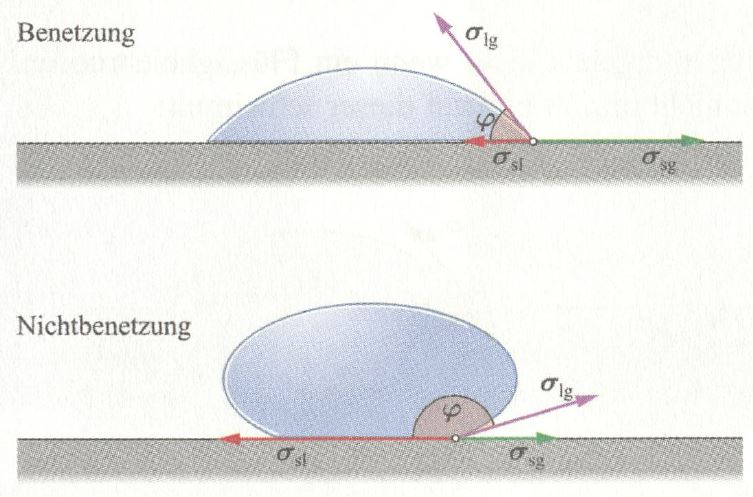
\includegraphics[width=7cm]{./bilder/Grenzflaechenspannung.jpg}
		\end{minipage}
		\newline
		\newline
		\newline
		\begin{minipage}[t]{12cm}
			\myparagraph{Kapillarität}
				\renewcommand{\arraystretch}{2.5}
				\begin{tabular}{ p{4cm} p{7cm}}
					$h = \dfrac{2 \sigma}{\rho gr}$	&	$\sigma$ = Oberflächenspannung in $\frac{N}{m}$\\
				\end{tabular}
				\renewcommand{\arraystretch}{1.5}
				\begin{tabular}{ p{4cm} p{7cm}}
					& $h$ = Steighöhe in m\\
					& $\rho$ = Dichte Flüssigkeit in $\frac{kg}{m^3}$\\
					& $r$ = Radius des Röhrchens in $m$\\
				\end{tabular}
				\renewcommand{\arraystretch}{1}
		\end{minipage}
		\begin{minipage}[t]{10cm}
			\vspace{-\ht\strutbox}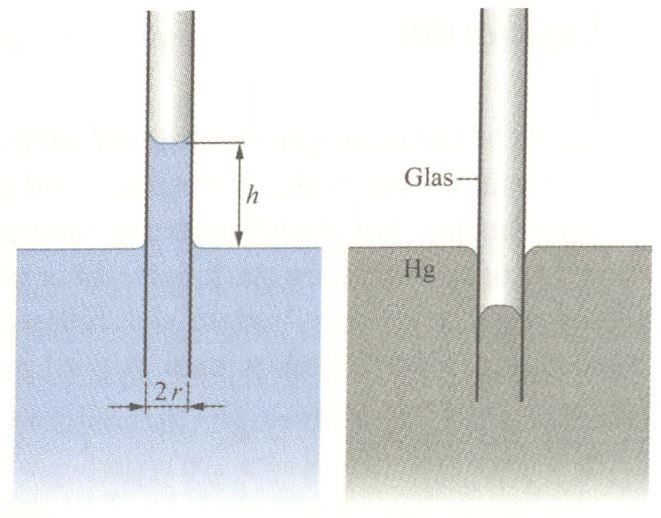
\includegraphics[width=7cm]{./bilder/Kapillaritaet.jpg}
		\end{minipage}
	

%%%%%%%%%%%%%%%%%%%%%%%%%%%%%%%%%%%%%%%%%%%%%%%%%%%%%%%%%%%%%%%%%%%%%%%%%%%%%%%%%%%%%%%%%%%%%%%%
% Hydrodynamik                                   
%%%%%%%%%%%%%%%%%%%%%%%%%%%%%%%%%%%%%%%%%%%%%%%%%%%%%%%%%%%%%%%%%%%%%%%%%%%%%%%%%%%%%%%%%%%%%%%%
\newpage
\subsection{Hydrodynamik}
	\subsubsection{Definitionen der Hydrodynamik}
		\begin{minipage}{19cm}
			\begin{itemize}
				\item \textbf{Abgeschlossene Fluidmenge:} ein Volumen, in welches keine Materie hinein oder heraus fliesst
				\item \textbf{Fluidteilchen:} ein materielles Fluidvolumen von sehr kleiner Ausdehnung
				\item \textbf{Geschwindigkeitsfeld:} ordnet jedem Punkt in einem Volumen eine Geschwindigkeit zu
				\item \textbf{Stationäre Strömung:} Geschwindigkeit, Druck, Dichte etc. ist zeitunabhängig
				\item \textbf{Stromlinie:} Kurven im Geschwindigkeitsfeld einer Strömung, deren Tangentenrichtung mit den Richtungen der Geschwindigkeitsvektoren übereinstimmen
				\item \textbf{Bahnlinie:} Eigentliche Bahn eines einzelnen Teilchens in einem Strömungsfeld
				\item \textbf{Laminare Strömung:} Strömung, in welcher die einzelnen Fluidteilchen sich in geordneten, nebeneinander gleitenden Schichten bewegen
				\item \textbf{Turbulente Strömung:} Strömung, in welcher Wirbel auftreten, wessen Kräfte entgegen der Bewegungsrichtung des Fluids wirken
			\end{itemize}
		\end{minipage}
	
	\subsubsection{Ideale Strömungen}
		\begin{minipage}{12cm}
			\myparagraph{Kontinuitätsgleichung (ideale Flüssigkeiten)}
				\begin{flushleft}
					Für eine inkompressible stationäre Strömung:
				\end{flushleft}
				\quad
				\renewcommand{\arraystretch}{2}
				\begin{tabular}{ p{5.5cm} p{7cm}}
					$\Delta m_1 = \Delta m_2$	&	$m$ = Masse in $kg$\\
					$\underbrace{\rho \cdot A_1 \cdot v_1 \cdot \Delta t}_{\Delta m_1} = \underbrace{\rho \cdot A_2 \cdot v_2 \cdot \Delta t}_{\Delta m_2}$	&	$\rho$ = Dichte Fluid in $\frac{kg}{m^3}$\\
					$A_1 \cdot v_1 = A_2 \cdot v_2$	&	$A$ = Querschnittsfläche Rohr in $m^2$\\
					$A \cdot v = konstant$	&	$v$ = Flussgeschwindigkeit Fluid in $\frac{m}{s}$\\
				\end{tabular}
				\renewcommand{\arraystretch}{1}
		\end{minipage}
		\begin{minipage}{10cm}
			\vspace{-\ht\strutbox}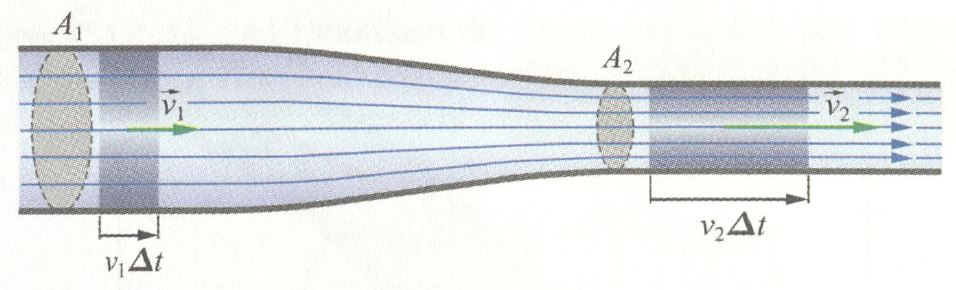
\includegraphics[width=7cm]{./bilder/Kontinuitaetsgleichung.jpg}
		\end{minipage}
		\newline
		\newline
		\newline
		\newline
		\begin{minipage}{12.5cm}
			\myparagraph{Bernoulli-Gleichung}
				\renewcommand{\arraystretch}{2.5}
				\begin{tabular}{ p{7.3cm} | p{4.5cm}}
					$\Delta W = \Delta W_{pot} + \Delta W_{kin}$	&	$\rho$ = Dichte Fluid in $\frac{kg}{m^3}$\\
					$W_{pot} = \underbrace{\rho \cdot A_2 \cdot \Delta s_2}_{\Delta m_2} \cdot g \cdot h_2 - \underbrace{\rho \cdot A_1 \cdot \Delta s_1}_{\Delta m_1} \cdot g \cdot h_1$	&	$A$ = Querschnittsfläche Rohr in $m^2$\\
					$W_{kin} = \underbrace{\rho \cdot A_2 \cdot \Delta s_2}_{\Delta m_2} \cdot \frac{1}{2} {v_2}^2 - \underbrace{\rho \cdot A_1 \cdot \Delta s_1}_{\Delta m_1} \cdot \frac{1}{2} {v_1}^2$	&	$s$ = von Fluid zurückgelegte Strecke in $m$\\
					$p_1 + \rho \cdot g \cdot h_1 + \rho \frac{{v_1}^2}{2} = p_2 + \rho \cdot g \cdot h_2 + \rho \frac{{v_2}^2}{2}$	&	$h_1$ = tiefer gelegener Rohrabschnitt in $m$\\
					$p + \rho \cdot g \cdot h + \rho \frac{{v}^2}{2} = konstant$	&	$h_2$ = höher gelegener Rohrabschnitt in $m$\\
				\end{tabular}
				\renewcommand{\arraystretch}{1.5}
				\begin{tabular}{ p{7.3cm} | p{7cm} }
					& $v$ = Flussgeschwindigkeit Fluid in $\frac{m}{s}$\\
				\end{tabular} 
				\renewcommand{\arraystretch}{1}
		\end{minipage}
		\begin{minipage}{10cm}
			\vspace{-\ht\strutbox}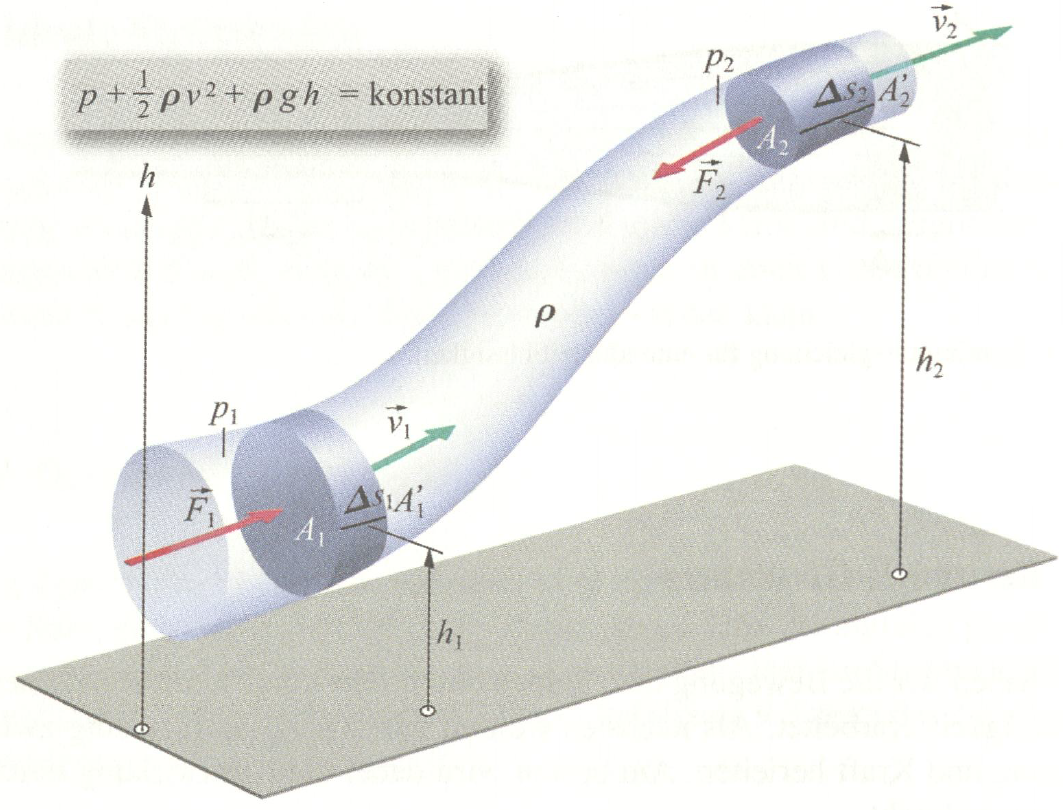
\includegraphics[width=7cm]{./bilder/BernoulliGleichung.png}
		\end{minipage}
		\newline
		\newline
		
		\myparagraph{Wirbelsatz von Thomson}
			\begin{minipage}{19cm}
				Die Zirkulation längs einer geschlossenen, materiellen Kurve in einem reibungsfreien, barotropen Fluid, auf das nur konservative Massenkräfte wirken, bleibt zeitlich konstant.
			\end{minipage}
		\newline
		\myparagraph{Wirbelsätze von Helmholtz}
			\begin{minipage}{19cm}
				\begin{enumerate}
					\item Die Zirkulation einer Wirbelröhre ist längs dieser Röhre konstant.
					\item Eine Wirbelröhre besteht immer aus denselben Fluidteilchen (wandert also mit).
					\item Die Zirkulation einer Wirbelröhre bleibt zeitlich konstant.
				\end{enumerate}
			\end{minipage}
		
		\subsubsection{Reale Strömungen}
			\begin{minipage}{12cm}
				\myparagraph{Newtonsches Reibungsgesetz}
				\begin{flushleft}
					Schubspannung: Spannung, welche eine an einem Körper parallel angreifende Kraft F verursacht.
				\end{flushleft}
				\renewcommand{\arraystretch}{2.5}
				\begin{tabular}{ p{4cm} | p{7cm}}
					$\tau = \dfrac{F_\parallel}{A} = \eta \dfrac{\mathrm{d}v}{\mathrm{d}z}$	&	$\tau$ = Schubspannung in $\frac{N \cdot s}{m^2} \cdot \frac{m}{s \cdot m} = \frac{N}{m^2}$\\
					$F_R = \eta \cdot A \frac{\mathrm{d}v}{\mathrm{d}y} = \tau \cdot A$ & $v$ = Geschwindigkeit Platte in $\frac{m}{s}$\\
				\end{tabular}
				\renewcommand{\arraystretch}{1.5}
				\begin{tabular}{ p{4cm} | p{10cm} }
					& $z$ = Dicke Fluidschicht in $m$\\
					& $A$ = parallel angreifende Fläche in $m^2$\\
					& $F_{\parallel} = F_R$ = parallel angreifende Reibungskraft in $N$\\
					& $\eta$ = dynamische Viskosität (Zähigkeit) in $\frac{kg}{ms} = \frac{N \cdot s}{m^2} = Pa \cdot s$\\
				\end{tabular} 
				\renewcommand{\arraystretch}{1}
			\end{minipage}
			\begin{minipage}{10cm}
				\vspace{-\ht\strutbox}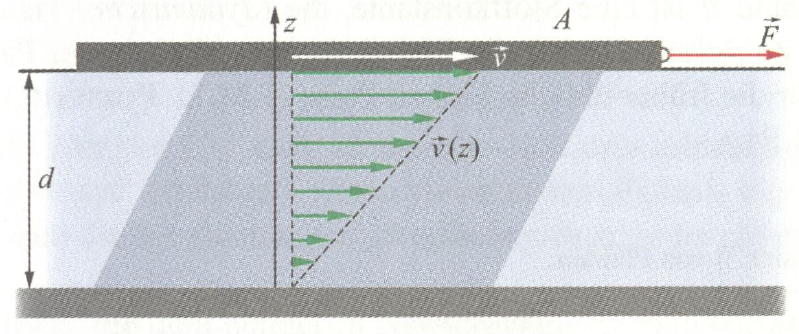
\includegraphics[width=7cm]{./bilder/NewtonschesReibungsgesetz.png}
			\end{minipage}
			\newline
			\newline
			\newline
			\newline
			\begin{minipage}{12cm}
				\myparagraph{Dynamische Viskosität (Zähigkeit), Fluidität}
				\renewcommand{\arraystretch}{2.5}
				\begin{tabular}{ p{4cm} | p{7cm}}
					$\eta = \tau \dfrac{\mathrm{d}z}{\mathrm{d}v}$	&	$\tau$ = Schubspannung in $\frac{N \cdot s}{m^2} \cdot \frac{m}{s \cdot m} = \frac{N}{m^2}$\\
					$\varphi = \frac{1}{\eta} = \dfrac{\mathrm{d}v}{\tau \cdot \mathrm{d}z}$	& $v$ = Geschwindigkeit in $\frac{m}{s}$\\
				\end{tabular}
				\renewcommand{\arraystretch}{1.5}
				\begin{tabular}{ p{4cm} | p{10cm} }
					& $z$ = Dicke Fluidschicht in $m$\\
					& $\eta$ = dynamische Viskosität (Zähigkeit) in $\frac{kg}{m \cdot s} = \frac{N \cdot s}{m^2} = Pa \cdot s$\\
					& $\varphi$ = Fluidität in $\frac{s^2}{kg \cdot m} \cdot m^2 \cdot \frac{m}{m \cdot s} = \frac{m \cdot s}{kg} = \frac{m^2}{N \cdot s} = \frac{1}{Pa \cdot s}$\\
				\end{tabular} 
				\renewcommand{\arraystretch}{1}
			\end{minipage}
			\newline
			\newline
			\newline
			\begin{minipage}[t]{16cm}
				\myparagraph{Reynoldszahl}
				\begin{flushleft}
					Einheitslose Zahl, welche den Übergang von einer laminaren in eine turbulente Strömung angibt.
				\end{flushleft}
				\renewcommand{\arraystretch}{2.5}
				\begin{tabular}{ p{6cm} | p{10cm}}
					$Re = \dfrac{\rho v d}{\eta}$	&	$Re$ = Reynoldszahl (Einheitslos)\\
					$Re_{krit} = 2320$	&	$\rho$ = Dichte Fluid in $\frac{kg}{m^3}$\\
					$Re < Re_{krit}$ \quad $\rightarrow$ laminare Strömung & $v$ = Geschwindigkeit Fluid in $\frac{m}{s}$\\
					$Re > Re_{krit}$ \quad $\rightarrow$ turbulente Strömung & $d$ = charakteristische Länge (bei Rohren meist Durchmesser)\\
				\end{tabular}
				\renewcommand{\arraystretch}{1.5}
				\begin{tabular}{ p{6cm} | p{10cm} }
					& $\eta$ = dynamische Viskosität (Zähigkeit) in $Pa \cdot s$\\
					& $Re_{krit}$ = kritische Reynoldszahl (Einheitslos)\\
				\end{tabular} 
				\renewcommand{\arraystretch}{1}
			\end{minipage}
			
			\myparagraph{Laminare Strömung}
			\newline
				\begin{minipage}{13cm}
					\textbf{Formel von Stokes}
						\begin{flushleft}
							Reibungswiderstand einer Kugel mit Radius R.
						\end{flushleft}
						\renewcommand{\arraystretch}{2.5}
						\begin{tabular}{ p{4cm} | p{7cm}}
							$F_R = 6 \pi \eta r v$	&	$F_R$ = Reibungskraft in $N$\\
							$F_G = F_R + F_A$	&	$\eta$ = dynamische Viskosität (Zähigkeit) in $Pa \cdot s$\\
							$\eta = \dfrac{r^2 g (\rho_K - \rho_{fl}) \cdot 2}{9 \cdot v}$	&	$r$ = Kugelradius in $m$\\
						\end{tabular}
						\renewcommand{\arraystretch}{1.5}
						\begin{tabular}{ p{4cm} | p{8cm} }
							& $\rho_{k}$ = Dichte Kugel in $\frac{kg}{m^3}$\\
							& $\rho_{fl}$ = Dichte Fluid in $\frac{kg}{m^3}$\\
							& $v$ = Strömungsgeschwindigkeit Fluid/Körper in $\frac{m}{s}$\\
						\end{tabular} 
						\renewcommand{\arraystretch}{1}
				\end{minipage}
				\begin{minipage}{10cm}
					\vspace{-\ht\strutbox}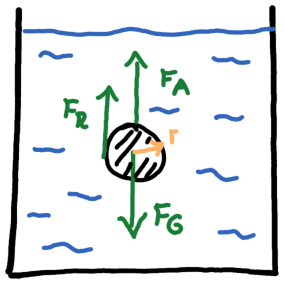
\includegraphics[width=5cm]{./bilder/StokesscheGleichung.png}
				\end{minipage}
				\newline
				\newline
				\newline
				\newline
				\begin{minipage}{12cm}
					\textbf{Laminare Rohrströmung (Gesetz von Hagen-Poiseuille)}
						\renewcommand{\arraystretch}{2.5}
						\begin{tabular}{ p{4cm} | p{7cm}}
							$V = \dfrac{\pi tR^4}{8 \eta l}\Delta p$	&	$V$ = geflossenes Fluidvolumen in $m^3$\\
							$\dfrac{dV}{dt} = \dfrac{\pi \overbrace{(p_1 - p_2)}^{\Delta p} R^4}{8 \eta l}$	& $R$ = Rohrradius in $m$\\
							$v(r) = -\dfrac{1}{4 \eta l} \cdot \Delta p \cdot (R^2-r^2)$ & $r$ = innerer Radius in Flüssigkeit in $m$\\
						\end{tabular}
						\renewcommand{\arraystretch}{1.5}
						\begin{tabular}{ p{4cm} | p{8cm} }
							& $\eta$ = dynamische Viskosität (Zähigkeit) in $Pa \cdot s$\\
							& $l$ = Länge des Rohres in $m$\\
							&	$\Delta p$ = Druckdifferenz zwischen Rohrenden in $Pa$\\
						\end{tabular} 
						\renewcommand{\arraystretch}{1}
				\end{minipage}
				\begin{minipage}{10cm}
					\vspace{-\ht\strutbox}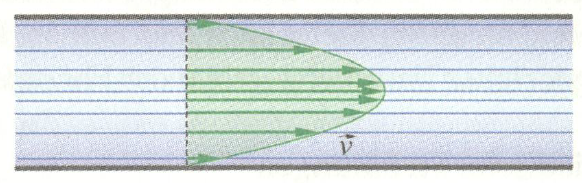
\includegraphics[width=6cm]{./bilder/Rohrstroemung1.png}
					\vspace{-\ht\strutbox}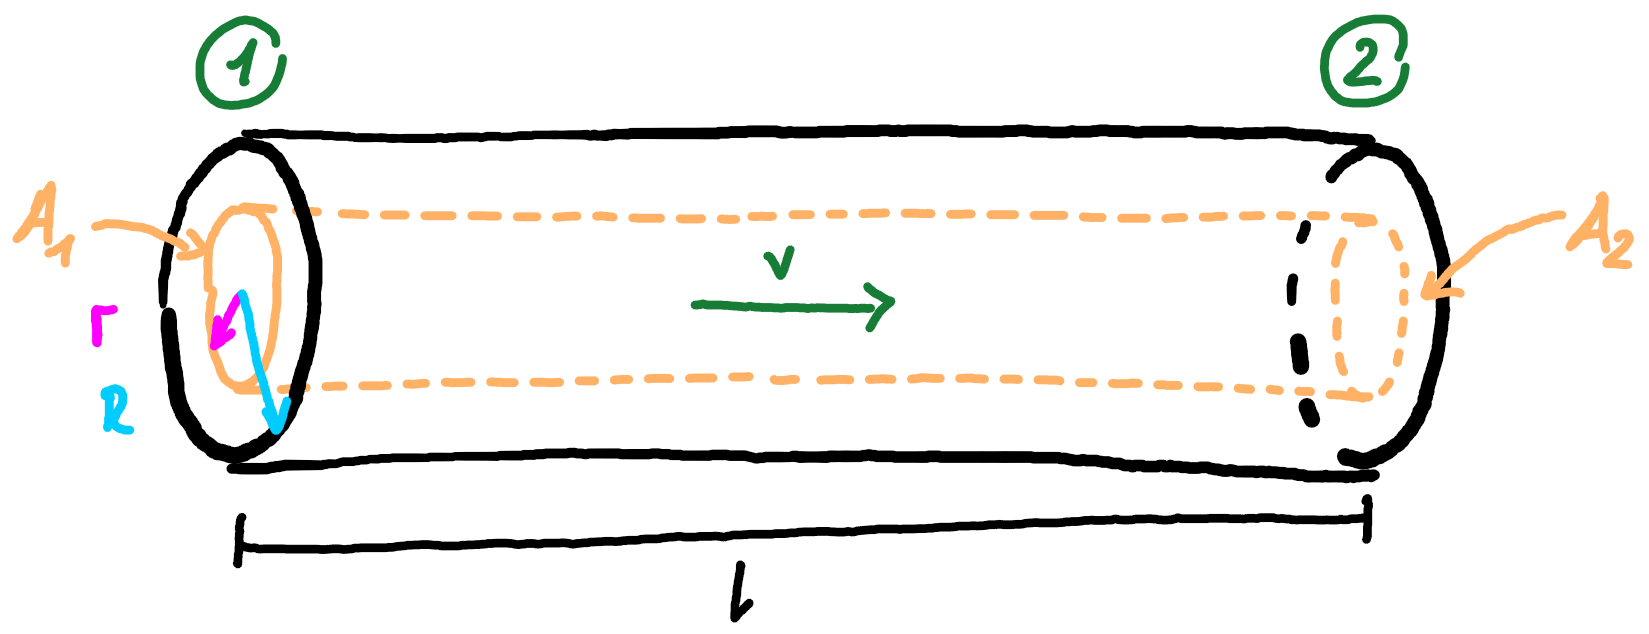
\includegraphics[width=6cm]{./bilder/Rohrstroemung2.png}
				\end{minipage}
				\newline
			\myparagraph{Turbulente Strömung}
			\newline
				\begin{minipage}{10.1cm}
					\textbf{Strömungswiderstand}
						\begin{flushleft}
						\end{flushleft}
						\renewcommand{\arraystretch}{2.5}
						\begin{tabular}{ p{3cm} | p{10cm}}
							$F_D = c_W A \dfrac{\rho v^2}{2}$	&	$F_D$ = Druckwiderstandskraft in $N$\\
							$F_W = c_W A_T \dfrac{\rho v^2}{2}$	&	$F_W$ = induzierte Widerstandskraft in $N$\\
							$F_A = c_A A_T \dfrac{\rho v^2}{2}$	&	$F_A$ = Auftriebskraft in $N$\\
							$c_W = \dfrac{F_W}{A}\dfrac{2}{\rho v^2}$	&	$c_W$ = Widerstandskoeffizient (Einheitslos)\\
						\end{tabular}
						\renewcommand{\arraystretch}{1.5}
						\begin{tabular}{ p{3cm} | p{10cm} }
							& $c_A$ = Auftriebskoeffizient (Einheitslos)\\
							& $\rho$ = Dichte Fluid in $\frac{kg}{m^3}$\\
							& $A$ = der Strömung entgegenstehender Körperquerschnitt in $m^2$\\
							& $A_T$ = zur Anströmrichtung parallele Ebene in $m^2$\\
							& $v$ = Strömungsgeschwindigkeit Fluid/Körper in $\frac{m}{s}$\\
						\end{tabular} 
						\renewcommand{\arraystretch}{1}
				\end{minipage}
				\begin{minipage}{10cm}
					\vspace{-\ht\strutbox}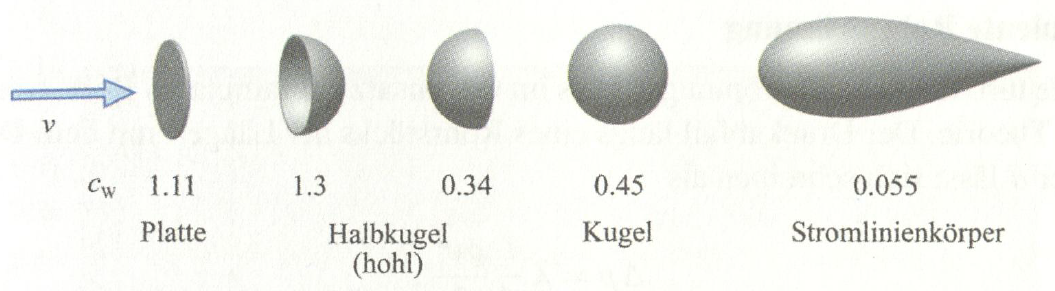
\includegraphics[width=9cm]{./bilder/WiderstandkoeffizientBeispiele.png}
				\end{minipage}
			
		\subsubsection{Dynamischer Auftrieb}
			\myparagraph{Magnus-Effekt}
				\newline
				Auftriebskraft, welche durch Rotation eines Körpers, welcher senkrecht von einer parallelen Strömung angeströmt wird, entsteht.
				\newline
				\newline
				\begin{minipage}[t]{13cm}
					\textbf{Zirkulation (für Zylinder)}
						\begin{flushleft}
							Mass für die Wirbelstärke in einer Strömung.
						\end{flushleft}
						\renewcommand{\arraystretch}{2.5}
						\begin{tabular}{ p{5cm} | p{7cm}}
							$\Gamma = \oint \vec{v} \cdot \mathrm{d} \vec{s} = 2 \pi r v_{Zyl} = 4 \pi^2 r^2 f$	&	$\Gamma$ = Zirkulation in $\frac{m^2}{s}$\\
						\end{tabular}
						\renewcommand{\arraystretch}{1.5}
						\begin{tabular}{ p{5cm} | p{7cm} }
							& $v$ = Anströmgeschwindigkeit Fluid in $\frac{m}{s}$\\
							& $v_{Zyl}$ = Umfangsgeschwindigkeit Zylinder in $\frac{m}{s}$\\
							& $f$ = Drehzahl Zylinder in $\frac{1}{s} = Hz$\\
						\end{tabular} 
						\renewcommand{\arraystretch}{1}
				\end{minipage}
				\begin{minipage}[t]{10cm}
					\vspace{-\ht\strutbox}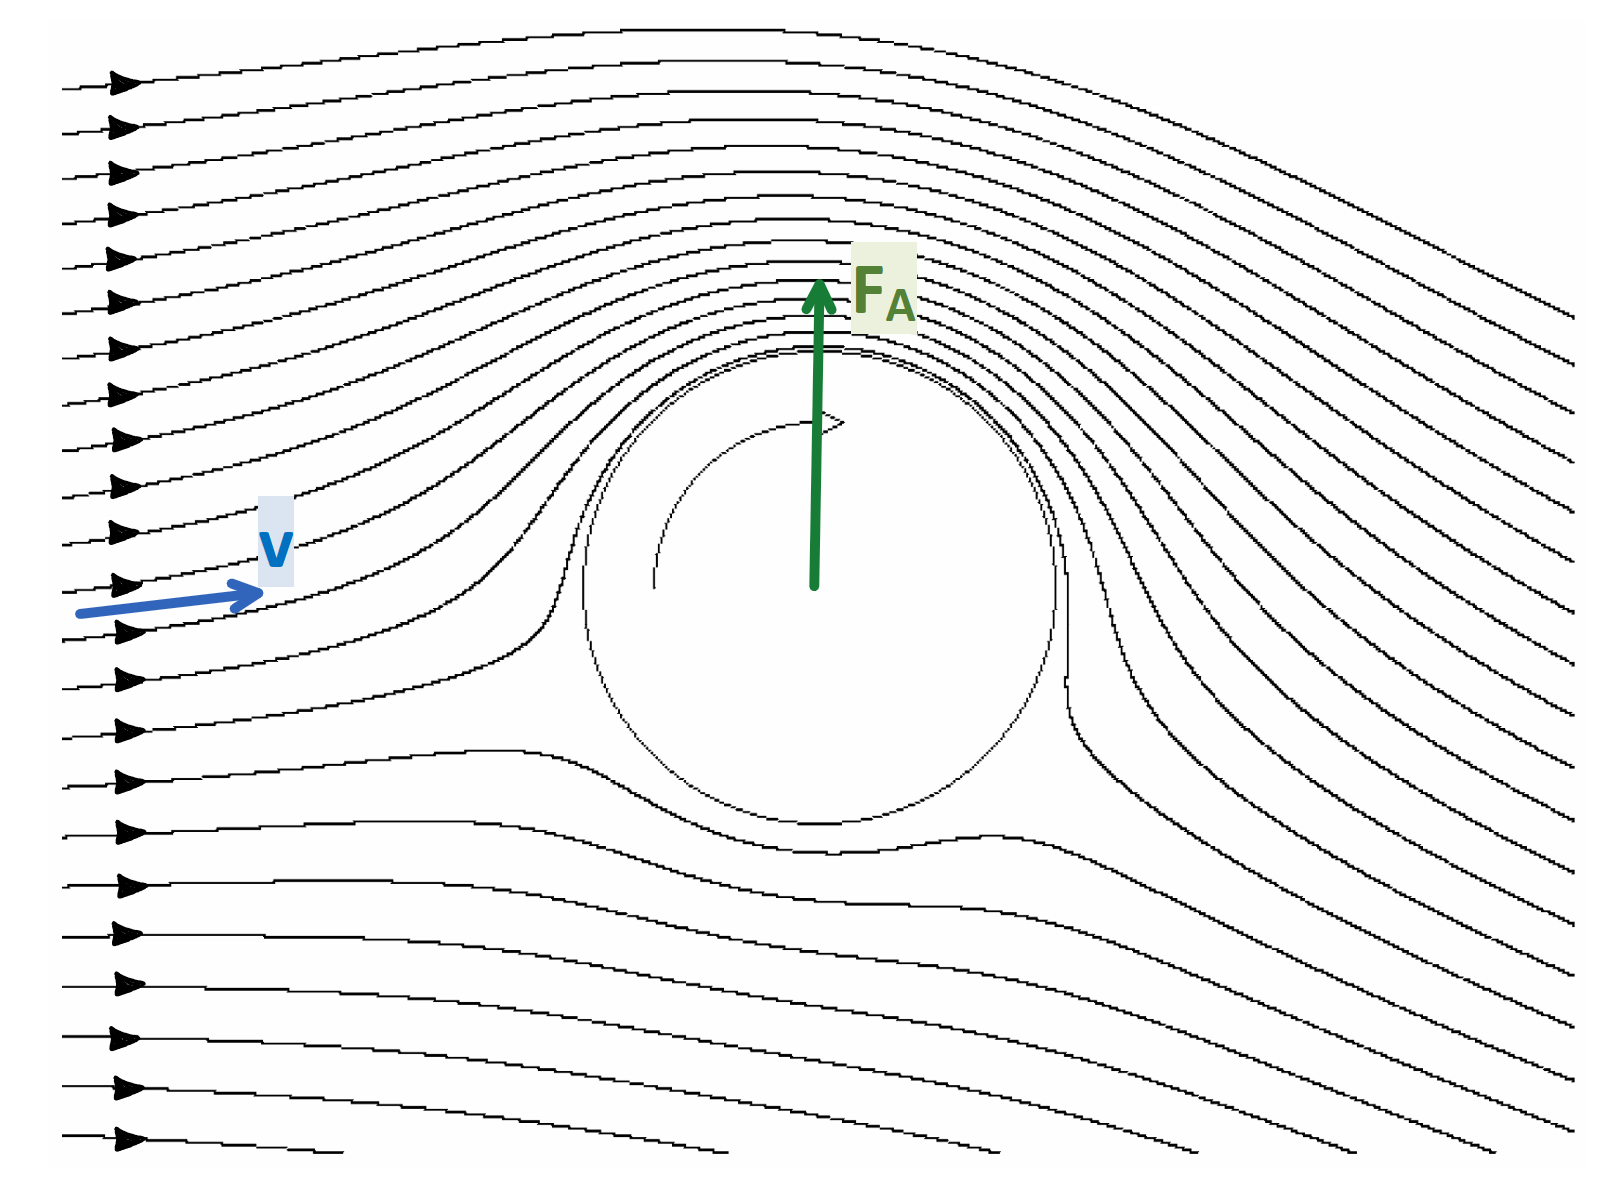
\includegraphics[width=6cm]{./bilder/MagnusEffekt.png}
				\end{minipage}
				\begin{minipage}[t]{13cm}
					\textbf{Kutta-Joukowski}
					\begin{flushleft}
						Proportionalität des dynamischen Auftriebs zur Zirkulation
					\end{flushleft}
					\renewcommand{\arraystretch}{2.5}
					\begin{tabular}{ p{5cm} | p{7cm}}
						$F_A = \rho lv \Gamma$	&	$F_A$ = Auftriebskraft in $N$\\
					\end{tabular}
					\renewcommand{\arraystretch}{1.5}
					\begin{tabular}{ p{5cm} | p{7cm} }
						& $\rho$ = Dichte Fluid in $\frac{kg}{m^3}$\\
						& $l$ = Länge Zylinder in $m$\\
						& $v$ = Anströmgeschwindigkeit Fluid in $\frac{m}{s}$\\
						& $\Gamma$ = Zirkulation in $\frac{m^2}{s}$
					\end{tabular} 
					\renewcommand{\arraystretch}{1}
				\end{minipage}
			


%%%%%%%%%%%%%%%%%%%%%%%%%%%%%%%%%%%%%%%%%%%%%%%%%%%%%%%%%%%%%%%%%%%%%%%%%%%%%%%%%%%%%%%%%%%%%%%%
% Wärmelehre                                   
%%%%%%%%%%%%%%%%%%%%%%%%%%%%%%%%%%%%%%%%%%%%%%%%%%%%%%%%%%%%%%%%%%%%%%%%%%%%%%%%%%%%%%%%%%%%%%%%
\newpage
\section{Wärmelehre}
	\subsection{Einführung Wärmelehre}
	\subsubsection{Definitionen der Wärmelehre}\label{DefinitionenDerWaermelehre}
		\begin{minipage}{18cm}
			\begin{itemize}
				\item \textbf{Wärme(-energie) $\boldsymbol{Q}$:} eine Form der Energie, welche dem Gesetz der Energieerhaltung unterliegt und welche aufgrund einer Temperaturdifferenz übertragen wird. Die Wärme fliesst stets von der höheren zur tieferen Temperatur. [$Q$] = Joule, Kalorie
				\item \textbf{Temperatur:} ein Mass für die Bewegungsenergie der Moleküle eines Körpers oder Fluids
				\item \textbf{Tripelpunkt:} Punkt, an welchem feste, flüssige und gasförmige Phasen im Gleichgewicht sind. Ist die Temperatur unter dem Tripelpunkt geht ein Stoff direkt vom festen in den gasförmigen Zustand über ohne flüssig zu werden. \label{Tripelpunkt}
				\item \textbf{Kritische Temperatur:} Temperatur, oberhalb welcher die Verflüssigung eines Gases auch bei noch so hohem Druck nicht mehr möglich ist \label{KritischTemperatur}
				\item \textbf{Siedepunkt:} Gleichgewichtstemperatur zwischen Wasser und Dampf bei einem Luftdruck von 101 325 Pa
				\item \textbf{Eispunkt:} Gleichgewichtstemperatur zwischen Eis und luftgesättigtem Wasser bei einem Luftdruck von 101 325 Pa
				\item \textbf{Stoffmenge $\boldsymbol{n}$:} quantitative Mengenangabe von Stoffen, basierend auf 12g C-12-Kohlenstoff. $n = 6.022 \cdot 10^{23}$ Moleküle; [$n$] = mol (SI-Einheit)
				\item \textbf{Avogadrokonstante $\boldsymbol{N_A}$:} Anzahl Atome/Moleküle, welche in der Stoffmenge von 1 Mol enthalten sind
				\item \textbf{Extensive Grössen:} hängen von der Substanzmenge ab (z.B. Volumen, Stoffmenge)
				\item \textbf{Intensive Grössen:} sind von der Substanzmenge unabhängig (z.B. Temperatur)
				\item \textbf{Spezifische Grössen:} sind extensive Grössen pro Stoffmenge (z.B. Volumen/mol)
				\item \textbf{Offenes System:} System mit Energie- und Materieaustausch
				\item \textbf{Geschlossenes System:} System mit Energie-, aber ohne Materieaustausch
				\item \textbf{Abgeschlossenes System:} System ohne Energie- und ohne Materieaustausch
				\item \textbf{Adiabatisch:} System mit Arbeitsaustausch (Zustandsänderung), aber ohne Wärme- und ohne Materieaustauch
				\item \textbf{Isobar:} konstanter Druck
				\item \textbf{Isochor:} konstantes Volumen
				\item \textbf{Isotherm:} konstante Temperatur
				\item \textbf{Homogenes System:} System, das an allen Stellen die gleichen Eigenschaften hat
				\item \textbf{Heterogenes System:} System, das aus Bereichen mit verschiedenen Eigenschaften besteht, wobei sich dies an Grenzflächen abrupt ändern.
				\item \textbf{Phase:} Phase ist ein physikalisch und chemisch homogener Bereich in einem heterogenen System
				\item  \textbf{Aggregatszustand:} Unterschiedliche Zustände eines Stoffes, die sich durch bloße Änderungen von Temperatur oder Druck ineinander umwandeln können.
				\item \textbf{Dispersion:} Eine aus zwei oder mehreren Phasen bestehende Mischung, bei der eine Substanz in einer anderen in feinster Form verteilt ist
			\end{itemize}
		\end{minipage}

	\subsubsection{Wärmeeinheiten}
		\begin{minipage}{14cm}
			\begin{tabular}{ p{4cm} | p{6cm} }
				$T_K = T_C + 273.15$
				& $T_K$ = Temperatur in K\\
				$T_F = T_C \cdot 1.8 + 32$
				& $T_F$ = Temperatur in $^\circ F$\\
				& $T_C$ = Temperatur in $^\circ C$
			\end{tabular} 
		\end{minipage}
	
	\subsection{Thermische Zustandsgleichungen}
	\subsubsection{Wärmeausdehnung}
		\begin{minipage}{14cm}
			\myparagraph{Längen-, Flächen und Volumenausdehnung}
			\newline
				\begin{tabular}{ p{1.5cm} p{4.5cm} | p{7.5cm} }
					Fest:
					& 1D: $\Delta l = \alpha \cdot l_0 \cdot \Delta T $
						& $\alpha$ = Längenausdehungskoeffizient in $\frac{1}{K}$\\
					& 2D: $\Delta A = 2\alpha \cdot A_0 \cdot \Delta T$
						& $\gamma$ = Volumenausdehungskoeffizient\\
						&& \quad \quad in $\frac{1}{K} \text{ (für isotrope Mat.)}$\\
					& 3D: $\Delta V = \underbrace{3\alpha}_{\gamma} \cdot V_0 \cdot \Delta T$
						& T = Temperatur in K\\
					Flüssig:
					& 3D: $\Delta V = \gamma \cdot V_0 \cdot \Delta T$\\
					Gasförmig:
						& 3D: $\Delta V = \gamma \cdot V_0 \cdot \Delta T$\\
				\end{tabular} 
		\end{minipage}
		\begin{minipage}{10cm}
			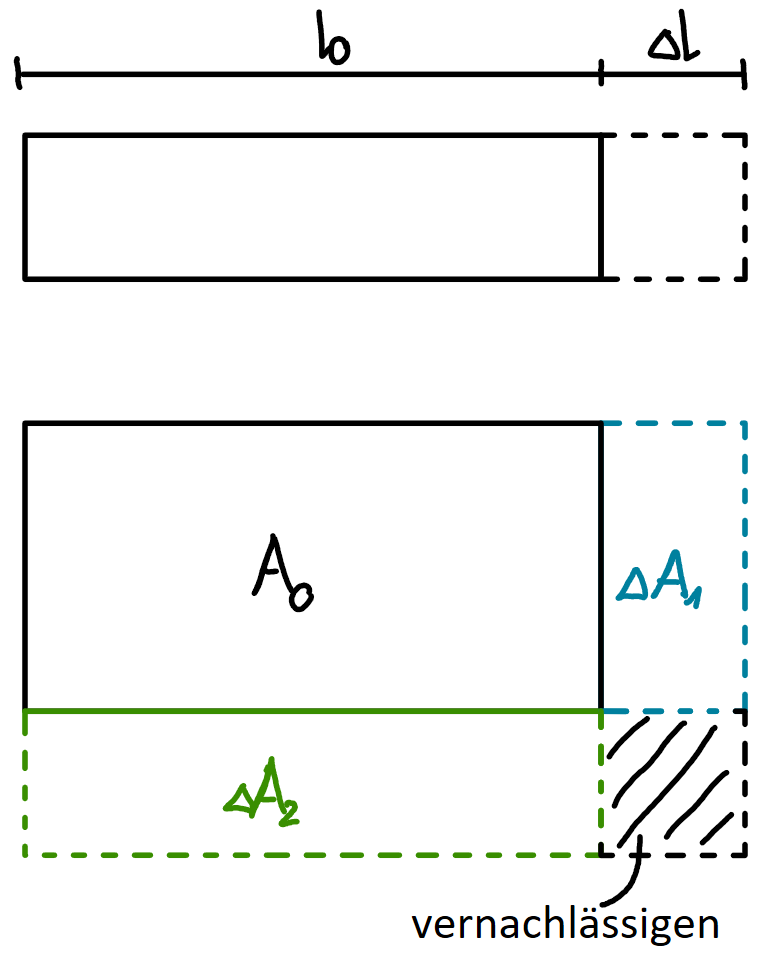
\includegraphics[width=3.5cm]{./bilder/Waermeausdehnung.png}
		\end{minipage}
		\begin{minipage}[t]{13cm}
			\myparagraph{Thermische Spannung (Hooksches Gesetz)}
			\begin{flushleft}
				Wird die thermische Ausdehnung behindert, treten mechanische Spannungen auf.
			\end{flushleft}
			\renewcommand{\arraystretch}{2}
			\begin{tabular}{ p{4cm} | p{7cm}}
				$\sigma = E \frac{\Delta l}{l_0} = E \alpha \Delta T$	&	$\sigma$ = thermische Spannung in $\frac{N}{m^2}$\\
				$\epsilon = \frac{\Delta l}{l_0}$	& $E$ = Elastizitätsmodul in $\frac{N}{m^2}$\\
			\end{tabular}
			\renewcommand{\arraystretch}{1.5}
			\begin{tabular}{ p{4cm} | p{7cm} }
				& $\alpha$ = Längenausdehnungskoeffizient in $\frac{1}{K}$\\
			\end{tabular} 
			\renewcommand{\arraystretch}{1}
		\end{minipage}

	\subsubsection{Ideale Gase}
		\begin{minipage}{15cm}
			\myparagraph{Eigenschaften idealer Gase}
				\begin{itemize}
					\item Die Moleküle sind Massenpunkte, d.h. sie haben eine Masse aber kein Volumen
					\item Es gibt keine intermolekularen Kräfte
					\item Die Gas-Temperatur ist weit höher als die kritische Temperatur
				\end{itemize}
				\renewcommand{\arraystretch}{1.5}
				\begin{tabular}{ | p{3cm} | p{4cm} | p{4cm} | p{4cm} |}
					\hline
					\textbf{Bezeichnung:} & \textbf{isobare} & \textbf{isochore} & \textbf{isotherme}\\
					\hline
				\end{tabular}
				\renewcommand{\arraystretch}{2}
				\begin{tabular}{ | p{3cm} | p{4cm} | p{4cm} | p{4cm} |}
					\textbf{Bedingung:} & p = konst & V = konst & T = konst\\
					\textbf{Formel:} & $\dfrac{V_1}{V_2} = \dfrac{T_1}{T_2}$ & $\dfrac{p_1}{p_2} = \dfrac{T_1}{T_2}$ & $\dfrac{p_1}{p_2} = \dfrac{V_2}{V_1}$\\
					\textbf{Gesetz:} & Gay-Lussac & Gay-Lussac & Boyle-Mariotte\\
					\hline
				\end{tabular}
				\renewcommand{\arraystretch}{1}
		\end{minipage}
		\newline
		\newline
		\newline
		\begin{minipage}{13cm}
			\myparagraph{Allgmeine Gasgleichung}
			\begin{flushleft}
				Avogadrosches Gesetz: Ideale Gase bei gleichem Druck und gleicher Temperatur enthalten in gleichen Volumina die gleiche Anzahl Moleküle.
			\end{flushleft}
			\renewcommand{\arraystretch}{2.5}
			\begin{tabular}{ p{5cm} | p{7cm}}
				$\dfrac{pV}{T} = konst$	&	$N$ = Anzahl Moleküle\\
				$pV = N k T = n \underbrace{N_A k}_R T = \dfrac{m}{M} R T$	&	$k$ = Boltzmann-Konstante = $1.381 \cdot 10^{-23} \frac{J}{K}$\\
			\end{tabular}
			\renewcommand{\arraystretch}{1.5}
			\begin{tabular}{ p{5cm} | p{7cm} }
				& $N_A$ = Avogadro-Konstante = $6.022 \cdot 10^{23}$\\
				& $n$ = Anzahl Mole\\
				& $R$ = Universelle Gaskonstante = $8.314 \frac{J}{mol \cdot K}$\\
				& $m$ = Masse vom Gas in $kg$\\
				& $M$ = Molmasse in $kg$\\
			\end{tabular} 
			\renewcommand{\arraystretch}{1}
		\end{minipage}
		\begin{minipage}{10cm}
			\vspace{-\ht\strutbox}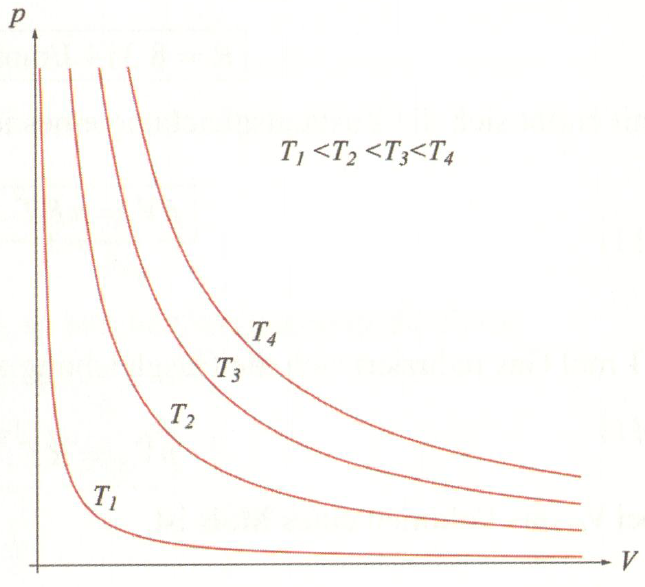
\includegraphics[width=6cm]{./bilder/Isotherme.png}
		\end{minipage}
		\newline
		\subsubsection{Gemische idealer Gase}
			\begin{minipage}[t]{10cm}
				\myparagraph{Gesetz von Dalton}
					\begin{flushleft}
						In einem Gasgemisch ist die Summe der Partialdrücke $p_i$ gleich dem Gesamtdruck $p$.
					\end{flushleft}
					\renewcommand{\arraystretch}{2.5}
					\begin{tabular}{ p{5cm} | p{7cm}}
						$p \cdot V = p(V_1 + V_2) = V(p_1 +p_2)$	&	$p_i$ = Partialdruck in $Pa$\\
						$p = \sum p_i$	& $p$ = Gesamtdruck in $Pa$\\
					\end{tabular}
					\renewcommand{\arraystretch}{1.5}
					\begin{tabular}{ p{5cm} | p{7cm}}
						& $V_i$ = Teilvolumen in $m^3$\\
						& $V$ = Gesamtvolumen in $m^3$\\
					\end{tabular} 
					\renewcommand{\arraystretch}{1}
			\end{minipage}
			\begin{minipage}[t]{10cm}
				\vspace{-\ht\strutbox}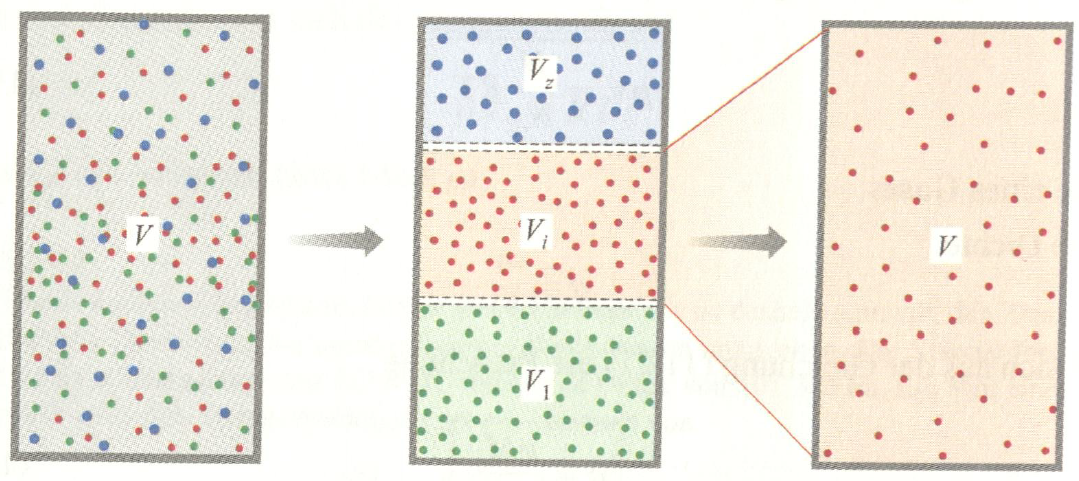
\includegraphics[width=9cm]{./bilder/GemischIdealerGase.png}
			\end{minipage}
		
	\subsubsection{Reale Gase}
		\begin{minipage}{15cm}
			\myparagraph{Eigenschaften realer Gase}
			\begin{itemize}
				\item Die Moleküle haben ein Eigenvolumen
				\item Es treten intermolekularen Kräfte auf
			\end{itemize}
		\end{minipage}
		\newline
		\newline
		\newline
		\newline
		\begin{minipage}{12.5cm}
			\myparagraph{Allgmeine Van der Waals'sche Zustandsgleichung}
				\newline
				\renewcommand{\arraystretch}{2.5}
				\begin{tabular}{ p{4cm} | p{7cm}}
					$p = \dfrac{nRT}{V-nb} - \dfrac{n^2 a}{V^2}$	&	$n$ = Anzahl Mole\\
				\end{tabular}
				\renewcommand{\arraystretch}{1.5}
				\begin{tabular}{ p{4cm} | p{7cm} }
					& $R$ = allgemeine Gaskonstante = $8.314 \frac{J}{mol \cdot K}$\\
					& $a, b$ = Van-der-Waals-Konstanten\\
				\end{tabular} 
				\renewcommand{\arraystretch}{1}
				\newline
				\newline
				\newline
				\textit{Achtung:} Das zwischen den Punkten A und D beschriebene Verhalten der Van der Waals'schen Zustandsgleichung ist unrealistisch. In der Realität bleibt der Druck zwischen den Punkten A und D konstant. Die Materie geht dabei vom gasförmigen in den flüssigen Zustand über.
		\end{minipage}
		\begin{minipage}{10cm}
			\vspace{-\ht\strutbox}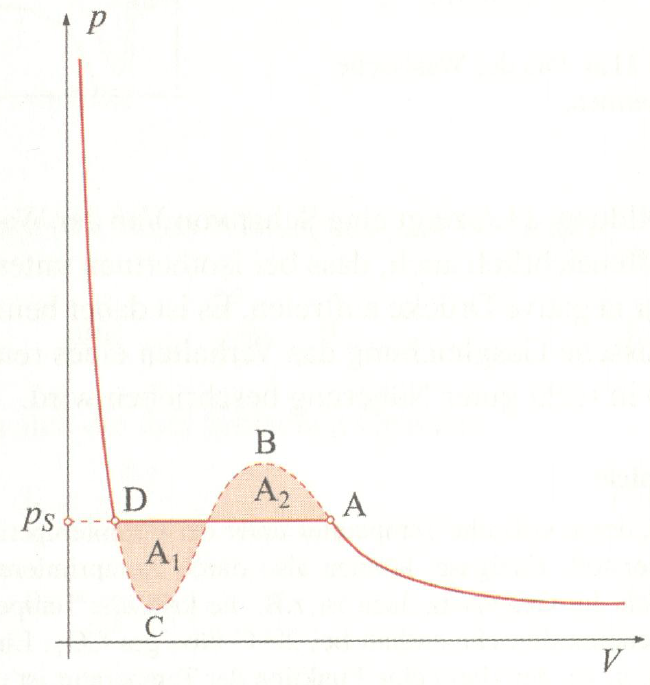
\includegraphics[width=6cm]{./bilder/VanDerWaalsscheZustandsfunktion.png}
		\end{minipage}
	\newpage
	\subsection{Kinetische Gastheorie}
		\begin{minipage}[t]{15cm}
			\subsubsection{Gasdruck}
				Die mittlere kinetische Energie der Moleküle ist proportional zur absoluten Temperatur.
				\newline
				\newline
				\renewcommand{\arraystretch}{2.5}
				\begin{tabular}{ p{4cm} | p{10cm}}
					$\overline{E_{kin}} = \dfrac{m\overline{v^2}}{2} = \dfrac{3}{2}kT$	&	$\overline{E_{kin}}$ = Mittlere kinetische Energie der Moleküle in $J$\\
				\end{tabular}
				\renewcommand{\arraystretch}{1.5}
				\begin{tabular}{ p{4cm} | p{7cm} }
					& $k$ = Boltzmannkonstannte =  $1.381 \cdot 10^{-23} \frac{J}{K}$\\
				\end{tabular} 
				\renewcommand{\arraystretch}{1}
		\end{minipage}
		\newline
		\newline
		\newline
		\newline
		\begin{minipage}[t]{10cm}
			\subsubsection{Äquipartiotionsgesetz}
				\renewcommand{\arraystretch}{2.5}
				\begin{tabular}{ p{2cm} | p{7cm}}
					$\overline{E} = \dfrac{f}{2}kT$	&	$\overline{E}$ = Gesamte mittlere Energie des Moleküls in $J$\\
				\end{tabular}
				\renewcommand{\arraystretch}{1.5}
				\begin{tabular}{ p{2cm} | p{7cm} }
					& $f$ = Anzahl Freiheitsgrade des Moleküls\\
					& $k$ = Boltzmannkonstannte =  $1.381 \cdot 10^{-23} \frac{J}{K}$\\
				\end{tabular} 
				\renewcommand{\arraystretch}{1}
		\end{minipage}
		\newline
		\newline
		\newline
		\newline
		\begin{minipage}[t]{18cm}
			\vspace{-\ht\strutbox}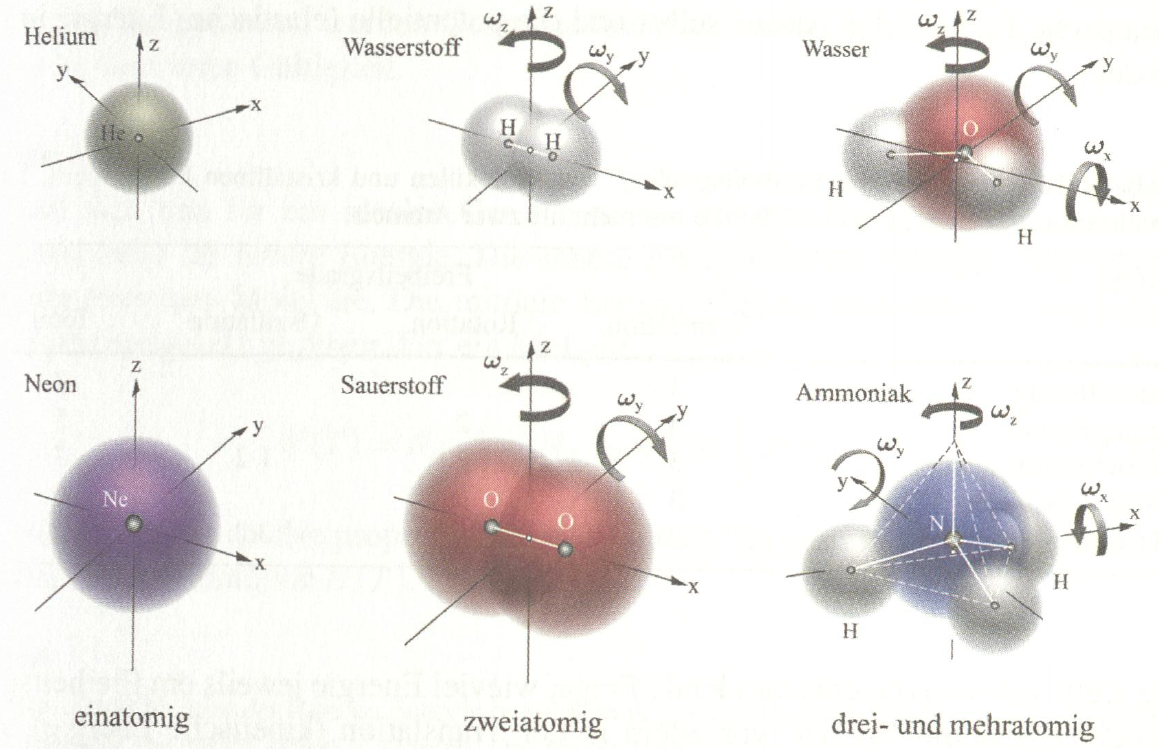
\includegraphics[width=10cm]{./bilder/FreiheitsgradeMolekuel.png}
		\end{minipage}
		\newline
		\newline
		\newline
		\newline
		\begin{minipage}{19cm}
			\renewcommand{\arraystretch}{1.5}
			\begin{tabular}{ | p{3cm} | p{13.28cm} |}
				\hline
				\textbf{Form:} & \textbf{Freiheitsgrade}\\
				\hline
			\end{tabular}
			\begin{tabular}{ | p{3cm} | p{3cm} | p{3cm} | p{3cm} | p{3cm} |}
				& Translation & Rotation & Oszillation & Total\\
				\hline
				Punktförmig & 3 & 0 & 0 & 3\\
				starre Hantel & 3 & 2 & 0 & 5\\
				schwingende Hantel & 3 & 2 & $1 \cdot 2$ & 7\\
				mehratomig starr & 3 & 3 & 0 & 6\\
				Kristall & 0 & 0 & $3 \cdot 2$ & 6\\
				\hline
			\end{tabular}
			\renewcommand{\arraystretch}{1}
			\vspace{3cm}
		\end{minipage}
		\newline
		\subsubsection{Maxwellsche Geschwindigkeitsverteilung}
		\begin{minipage}[t]{13cm}
			\myparagraph{Wahrscheinlichste Geschwindigkeit}
			\newline
			\renewcommand{\arraystretch}{2.5}
			\begin{tabular}{ p{3cm} | p{9cm}}
				$v_0 = \sqrt{\dfrac{2kT}{m}}$	&	$v_0$ = Wahrscheinlichste Geschwindigkeit in $\frac{m}{s}$\\
			\end{tabular}
			\renewcommand{\arraystretch}{1.5}
			\begin{tabular}{ p{3cm} | p{9cm} }
				& $k$ = Boltzmannkonstannte =  $1.381 \cdot 10^{-23} \frac{J}{K}$\\
			\end{tabular} 
			\renewcommand{\arraystretch}{1}
		\end{minipage}
		\newline
		\newline
		\newline
		\begin{minipage}[t]{13cm}
			\myparagraph{Mittlere Geschwindigkeit}
			\newline
			\renewcommand{\arraystretch}{2.5}
			\begin{tabular}{ p{3cm} | p{9cm}}
				$\overline{v} = \sqrt{\dfrac{8kT}{\pi m}}$	&	$\overline{v}$ = Mittlere Geschwindigkeit in $\frac{m}{s}$\\
			\end{tabular}
			\renewcommand{\arraystretch}{1.5}
			\begin{tabular}{ p{3cm} | p{9cm} }
				& $k$ = Boltzmannkonstannte =  $1.381 \cdot 10^{-23} \frac{J}{K}$\\
			\end{tabular} 
			\renewcommand{\arraystretch}{1}
		\end{minipage}
		\newline
		\newline
		\newline
		\begin{minipage}[t]{13cm}
			\myparagraph{Mittlere quadratische Geschwindigkeit}
			\newline
			\renewcommand{\arraystretch}{2.5}
			\begin{tabular}{ p{3cm} | p{9cm}}
				$u = \sqrt{\overline{v^2}}$ & $\overline{v}$ = Mittlere Geschwindigkeit in $\frac{m}{s}$\\
				$u = \sqrt{\dfrac{3kT}{m}}$	&	$u$ = mittlere quadratische Geschwindigkeit in $\frac{m}{s}$\\
			\end{tabular}
			\renewcommand{\arraystretch}{1.5}
			\begin{tabular}{ p{3cm} | p{9cm} }
				& $k$ = Boltzmannkonstannte =  $1.381 \cdot 10^{-23} \frac{J}{K}$\\
			\end{tabular} 
			\renewcommand{\arraystretch}{1}
		\end{minipage}
		\newline
		\newline
		\newline
		\subsubsection{Kinematik des Gases}
		\begin{minipage}[t]{13cm}
			\myparagraph{Mittlere freie Weglänge}
			\newline
			\renewcommand{\arraystretch}{2.5}
			\begin{tabular}{ p{3cm} | p{9cm}}
				$\overline{l} = \dfrac{1}{\sqrt{2}n\pi d^2}$	&	$l$ = mittlere freie Weglänge in $m$\\
			\end{tabular}
			\renewcommand{\arraystretch}{1.5}
			\begin{tabular}{ p{3cm} | p{9cm} }
				& $d$ = Molekül-Durchmesser in $m$\\
				& $n$ = Anzahl Moleküle pro Volumeneinheit\\
			\end{tabular} 
			\renewcommand{\arraystretch}{1}
		\end{minipage}
	
		\subsubsection{Transportvorgänge}
			\begin{minipage}{12cm}
				\myparagraph{Viskosität}
					\newline
					\renewcommand{\arraystretch}{2.5}
					\begin{tabular}{ p{4cm} | p{7cm}}
						$\eta = \dfrac{1}{3} \overline{v} \overline{l} \rho$	&	$\eta$ = Viskosität in $Pa \cdot s = \frac{N \cdot s}{m^2}$\\
					\end{tabular}
					\renewcommand{\arraystretch}{1.5}
					\begin{tabular}{ p{4cm} | p{10cm} }
						& $\overline{v}$ = Mittlere Geschwindigkeit in $\frac{m}{s}$\\
						& $\overline{l}$ = mittlere freie Weglänge in $m$\\
						& $\rho$ = Dichte Fluid in $\frac{kg}{m^3}$\\
					\end{tabular} 
					\renewcommand{\arraystretch}{1}
			\end{minipage}
	\newpage
	\subsection{Wärme}
		\begin{minipage}[t]{18cm}
			\subsubsection{Erster Hauptsatz der Thermodynamik}
				\begin{enumerate}
					\item  Die Innere Energie U ist die gesamte in einem System enthaltene Energie.
					\item Die Zunahme der inneren Energie eines thermodynamischen Systems ist gleich der Summe der von aussen zugeführten Arbeit und der von aussen zugeführt Wärme
				\end{enumerate}
				\renewcommand{\arraystretch}{2.5}
				\begin{tabular}{ p{5cm} | p{7cm}}
					$\mathrm{d} U = \delta W + \delta Q$	&	$U$ = Innere Energie in $J$\\
					$Q_{Ab} = Q_{Zu}$	& $W$ = Arbeit in $J$\\
				\end{tabular}
				\renewcommand{\arraystretch}{1.5}
				\newline
				\begin{tabular}{ p{5cm} | p{7cm} }
					& $Q$ = Wärme in $J$\\
					& $Q_{Ab}$ = Abgegebene Wärme in $J$\\
					& $Q_{Zu}$ = Zugeführte Wärme in $J$\\
				\end{tabular} 
				\renewcommand{\arraystretch}{1}
		\end{minipage}
		\newline
		\newline
		\newline
		\begin{minipage}[t]{18cm}
			\subsubsection{Spezifische und molare Wärmekapazität}
				\renewcommand{\arraystretch}{2.5}
				\begin{tabular}{ p{5cm} | p{7cm}}
					$c = \dfrac{C}{m}$	&	$c$ = spezifische Wärmekapazität in $\frac{J}{kg \cdot K}$\\
					$Q = c \cdot m \cdot \Delta T$	&	$C$ = Wärmekapazität in $\frac{J}{K}$\\
					$C_m = \dfrac{c}{n} = \dfrac{M \cdot C}{m} = M \cdot c$ & $C_m$ = molare Wärmekapazität in $\frac{J}{mol \cdot K}$
				\end{tabular}
				\renewcommand{\arraystretch}{1.5}
				\newline
				\begin{tabular}{ p{5cm} | p{7cm} }
					& $Q$ = Wärme in $J$\\
					& $n$ = Stoffmenge = Anzahl Mol\\
					& $M$ = Molmasse in $kg$\\
				\end{tabular} 
				\renewcommand{\arraystretch}{1}
		\end{minipage}
		\newline
		\newline
		\newline
		\begin{minipage}[t]{18cm}
			\subsubsection{Verbrennungsenergie}
				\renewcommand{\arraystretch}{2.5}
				\begin{tabular}{ p{5cm} | p{7cm}}
					$H_f = \dfrac{Q}{m}$	&	$H_f$ = Heizwert in $\frac{J}{kg}$\\
					$H_g = \dfrac{Q}{V}$	&	$H_G$ = Brennwert in $\frac{J}{m^3}$\\
				\end{tabular}
				\renewcommand{\arraystretch}{1.5}
				\newline
				\begin{tabular}{ p{5cm} | p{7cm} }
					& $Q$ = Wärme in $J$\\
				\end{tabular} 
				\renewcommand{\arraystretch}{1}
		\end{minipage}
		\newline
		\newline
		\newline
		\begin{minipage}[t]{18cm}
			\subsubsection{Mischtemperatur}
			\renewcommand{\arraystretch}{2.5}
			\begin{tabular}{ p{5cm} | p{7cm}}
				$T_{end} = \dfrac{m_1 \cdot c_1 \cdot T_1 + m_2 \cdot c_2 \cdot T_2}{m_1 \cdot c_1 + m_2 \cdot c_2}$	&	$T_{end}$ = Mischtemperatur in $K$\\
			\end{tabular}
			\renewcommand{\arraystretch}{1.5}
			\newline
			\begin{tabular}{ p{5cm} | p{7cm} }
				&	$c_i$ = spezifische Wärmekapazität in $\frac{J}{kg \cdot K}$\\
			\end{tabular} 
			\renewcommand{\arraystretch}{1}
		\end{minipage}
	
	\newpage
	\subsection{Phasen und Phasenübergänge}
		\begin{minipage}[t]{13cm}
			\subsubsection{Phasenübergänge}
			\renewcommand{\arraystretch}{2.5}
			\begin{tabular}{ p{4cm} | p{7cm}}
				$q_f = \dfrac{Q_f}{m}$	&	$q_f$ = spezifische Schmelzwärme in $\frac{J}{kg}$\\
				$q_s = \dfrac{Q_s}{m}$	&	$q_s$ = spezifische Verdampfungswärme in $\frac{J}{kg}$\\
			\end{tabular}
			\renewcommand{\arraystretch}{1.5}
			\begin{tabular}{ p{4cm} | p{7cm} }
				& $Q_f$ = Schmelzwärme in $J$\\
				& $Q_s$ = Verdampfungswärme in $J$\\
			\end{tabular} 
			\renewcommand{\arraystretch}{1}
		\end{minipage}
		\newline
		\newline
		\newline
		\begin{minipage}[t]{9cm}
			\subsubsection{Phasendiagramm}
			\vspace{0.5cm}
			\vspace{-\ht\strutbox}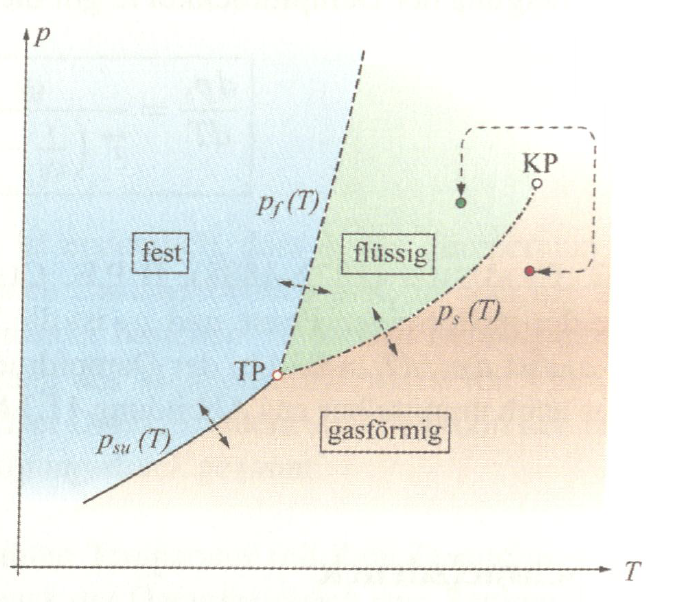
\includegraphics[width=7cm]{./bilder/Phasendiagramm.png} \\
			TP = Tripelpunkt\\
			KP = Krititische Temperatur\\
			(für Begriffserklärung siehe Kap. \ref{DefinitionenDerWaermelehre} \nameref{DefinitionenDerWaermelehre})
		\end{minipage}
		\begin{minipage}[t]{10cm}
			\subsubsection{Phasenübergangsdiagramm}
			\vspace{0.5cm}
			\vspace{-\ht\strutbox}\includegraphics[width=8.3cm]{./bilder/Phasenuebergangsdiagramm.png}
		\end{minipage}
		\vspace{1cm}
		\subsubsection{Luftfeuchtigkeit}
			\begin{minipage}[t]{13cm}
				\myparagraph{Formeln von Magnus}
					\renewcommand{\arraystretch}{3}
					\begin{tabular}{ p{6.5cm} | p{9cm}}
						$\vartheta \geq 0 $\textdegree$ C$: \quad $p_s = p_{s0} \cdot 10^{\frac{7.5 \vartheta}{\vartheta +237}}$	&	$\vartheta$ = Temperatur in \textdegree $C$\\
						$\vartheta \leq 0 $\textdegree$ C$: \quad $p_s = p_{s0} \cdot 10^{\frac{9.5 \vartheta}{\vartheta +265.5}}$	&	$\vartheta_d$ = Taupunkts-Temperatur in \textdegree $C$\\
						$p_s \geq 6.107hPa$: \quad $\vartheta = \dfrac{237 \cdot \log{(\frac{p_s}{6.107})}}{7.5 - \log{(\frac{p_s}{6.107})}}$	&	$p_s$ = Sättigungsdruck in $hPa$\\
						$p_s \leq 6.107hPa$: \quad $\vartheta = \dfrac{265.5 \cdot \log{(\frac{p_s}{6.107}})}{9.5 - \log{(\frac{p_s}{6.107})}}$	&	$p_{s0}$ = Dampfdruck in $hPa$ $(= 6.107hPa$ bei $0 $\textdegree$ C)$\\
						$\vartheta_d = \dfrac{237 \cdot (\log{(f_r)} + \frac{7.5 \cdot \vartheta}{\vartheta +237})}{7.5 - (\log{(f_r)} + \frac{7.5 \cdot \vartheta}{\vartheta +237})}$	& $f_r$ = relative Luftfeuchtigkeit (dimensionslos)\\
					\end{tabular}
					\renewcommand{\arraystretch}{1}
			\end{minipage}

	\newpage
	\subsection{Wärmetransport}
		\subsubsection{Wärmeleitung}
			\begin{minipage}[t]{16cm}
				\myparagraph{Fouriersches Gesetz der Wärmeleitung (Stationär (Zeitunabhängig))}
					\renewcommand{\arraystretch}{2.5}
					\begin{tabular}{ p{4cm} | p{7cm}}
						$j = -\lambda \dfrac{\mathrm{d}T}{\mathrm{d}x}$	&	$j$ = Wärmestromdichte in $\frac{W}{m^2}$\\
					\end{tabular}
					\renewcommand{\arraystretch}{1.5}
					\begin{tabular}{ p{4cm} | p{7cm} }
						& $\lambda$ = Wärmeleitfähigkeit in $\frac{W}{m \cdot K}$\\
						& $x$ = Distanz in x-Richtung in $m$\\
					\end{tabular} 
					\renewcommand{\arraystretch}{1}
			\end{minipage}
		\newline
		\newline
		\begin{minipage}[t]{13cm}
			\subsubsection{Wärmeleitungsgleichung (Instationär (Zeitabhängig))}
				\renewcommand{\arraystretch}{2.5}
				\begin{tabular}{ p{4cm} | p{7cm}}
					$\dfrac{\partial T}{\partial t} = \underbrace{\dfrac{\lambda}{\rho c}}_a \cdot \dfrac{\partial^2 T}{\partial x^2}$	& $\lambda$ = Wärmeleitfähigkeit in $\frac{W}{m \cdot K}$\\
				\end{tabular}
				\renewcommand{\arraystretch}{1.5}
				\begin{tabular}{ p{4cm} | p{7cm} }
					& $x$ = Distanz in x-Richtung in $m$\\
					& $\rho$ = Materialdichte in $kg/m^3$\\
					& $c$ = spezifische Wärmekapazität in $\frac{J}{kg \cdot K}$\\
					& $a$ = Temperaturleitfähigkeit in $\frac{m^2}{s}$
				\end{tabular} 
				\renewcommand{\arraystretch}{1}
		\end{minipage}
		\newline
		\newline
		\begin{minipage}[t]{11.5cm}
			\subsubsection{Wärmeübergang}
				\renewcommand{\arraystretch}{2.5}
				\begin{tabular}{ p{4cm} | p{7cm}}
					$j = \alpha(T_w -T)$	&	$j$ = Wärmestromdichte in $\frac{W}{m^2}$\\
				\end{tabular}
				\renewcommand{\arraystretch}{1.5}
				\begin{tabular}{ p{4cm} | p{7cm} }
					& $\alpha$ = Wärmeübergangszahl in $\frac{W}{m^2 \cdot K}$\\
					& $T_w$ = Temperatur an der Wand in $K$\\
					& $T$ = Umgebungstemperatur in $K$\\
				\end{tabular} 
				\renewcommand{\arraystretch}{1}
		\end{minipage}
		\begin{minipage}[t]{10cm}
			\vspace{-\ht\strutbox}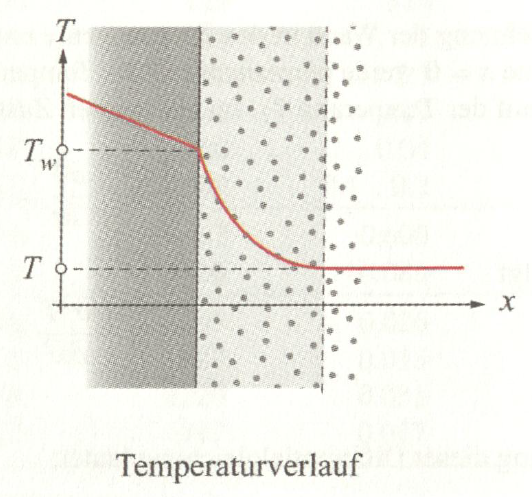
\includegraphics[width=5.5cm]{./bilder/Waermeuebergang.png}
		\end{minipage}
		\newline
		\newline
		\newline
		\newline
		\begin{minipage}{12cm}
			\myparagraph{Typische Wärmeübergangszahlen für Gebäude}
			\newline
			\renewcommand{\arraystretch}{1.5}
			\begin{tabular}{ | p{5cm} | p{3cm} |}
				\hline
				\textbf{an} & $\boldsymbol{\alpha}$ in $\frac{W}{m^2 \cdot K}$\\
				\hline
				Wandflächen & \\
				\quad innen & 8\\
				\quad aussen & 20\\
				\hline
				Böden und Decken & \\
				\quad Wärmestrom nach oben & 8\\
				\quad Wärmestrom nach unten & 6\\
				\hline
			\end{tabular}
			\renewcommand{\arraystretch}{1}
		\end{minipage}
		\vspace{3cm}
		\newline
		\subsubsection{Wärmedurchgang}
			\begin{minipage}{12cm}
				\myparagraph{Wärmedurchgang durch ebene (mehrschichtige) Wand}
					\renewcommand{\arraystretch}{2.5}
					\begin{tabular}{ p{4cm} | p{7cm}}
						$k = \dfrac{1}{\dfrac{1}{\alpha_i} + \sum\limits_{s}\dfrac{d_s}{\lambda_s} + \dfrac{1}{\alpha_a}}$	&	$k$ = k-Wert, Wärmedurchgangszahl in $\frac{W}{m^2 \cdot K}$\\
						$j = k \Delta T$	&	$\alpha_i$ = Wärmeübergangszahl innen in $\frac{W}{m^2 \cdot K}$\\
						$P = k \cdot A \cdot \Delta T$	& $\alpha_a$ = Wärmeübergangszahl aussen in $\frac{W}{m^2 \cdot K}$\\
					\end{tabular}
					\renewcommand{\arraystretch}{1.5}
					\begin{tabular}{ p{4cm} | p{7cm} }
						& $d_s$ = Wandstärke Schicht s in $m$\\
						& $\lambda_s$ = Wärmeleitfähigkeit Schicht s in $\frac{W}{m \cdot K}$\\
						& $j$ = Wärmestromdichte in $\frac{W}{m^2}$\\
						& $P$ = Wärmeleistung in $W$\\
					\end{tabular} 
					\renewcommand{\arraystretch}{1}
			\end{minipage}
			\begin{minipage}{10cm}
				\vspace{-\ht\strutbox}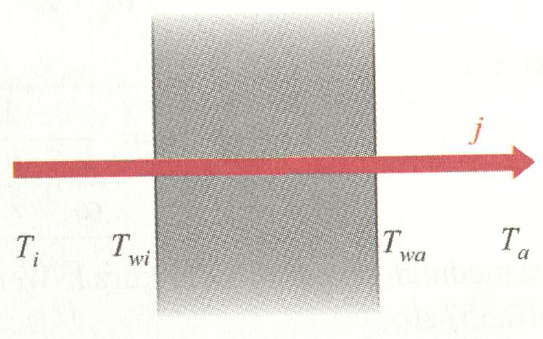
\includegraphics[width=6.5cm]{./bilder/Waermedurchgang.png}
			\end{minipage}
			\newline
			\newline
			\newline
			\newline
			\begin{minipage}{12cm}
				\myparagraph{Wärmedurchgang durch kreiszylindrische (mehrschichtige) Wand}
					\renewcommand{\arraystretch}{2.5}
					\begin{tabular}{ p{7cm} | p{7cm}}
						$k_a = \dfrac{1}{r_a} \cdot \dfrac{1}{\dfrac{1}{r_i \alpha_i} + \sum\limits_{s}\dfrac{1}{\lambda_s} \ln(\dfrac{r_{sa}}{r_{si}}) + \dfrac{1}{r_a \alpha_a}}$	&	$k_a$ = k-Wert, Wärmedurchgangszahl in $\frac{W}{m^2 \cdot K}$\\
					\end{tabular}
					\renewcommand{\arraystretch}{1.5}
					\begin{tabular}{ p{7cm} | p{7cm} }
						& $r_i$ = Innenradius in $m$\\
						& $r_a$ = Aussenradius in $m$\\
						& $r_{si}$ = Innenradius Schicht s in $m$\\
						& $r_{sa}$ = Aussenradius Schicht s in $m$\\
						& $\alpha_i$ = Wärmeübergangszahl innen in $\frac{W}{m^2 \cdot K}$\\
						& $\alpha_a$ = Wärmeübergangszahl aussen in $\frac{W}{m^2 \cdot K}$\\
						& $\lambda_s$ = Wärmeleitfähigkeit Schicht s in $\frac{W}{m \cdot K}$\\
					\end{tabular} 
					\renewcommand{\arraystretch}{1}
			\end{minipage}
			\newline
			\newline
			\newline
			\begin{minipage}[t]{13cm}
				\subsubsection{Wärmebedarf eines Gebäudes}
					\renewcommand{\arraystretch}{2.5}
					\begin{tabular}{ p{5cm} | p{13cm}}
						$Q_{tot} = Q_W + Q_L$	&	$Q_{tot}$ = totale Wärme in $J$\\
						$Q_W = A \cdot k \cdot t \cdot \Delta T$	&	$Q_W$ = Wärmefluss durch alle Wände in $J$\\
						$Q_L = c_l \cdot \rho_l \cdot \dfrac{V}{t} \Delta T $	&	$Q_L$ = Wärmefluss durch Lüftung in $J$\\
						$Q = (\sum\limits_{w} A_W k_W + \rho \cdot c_l \cdot \dfrac{V}{t}) G$ & $A$ = Wandfläche in $m^2$\\
					\end{tabular}
					\renewcommand{\arraystretch}{1.5}
					\begin{tabular}{ p{5cm} | p{13cm} }
						& $j$ = Wärmestromdichte in $\frac{W}{m^2}$\\
						& $k_a$ = k-Wert, Wärmedurchgangszahl in $\frac{W}{m^2 \cdot K}$\\
						& $c_l$ = spezifische Wärmekapazität in $\frac{J}{kg \cdot K}$\\
						& $\rho_l$ = Luftdichte in $\frac{kg}{m^3}$\\
						& $V$ = Raumvolumen in $m^3$\\
						& $t$ = Dauer des Luftwechsels in $s$ (Bsp. 2-facher Luftwechsel pro Stunde $= \frac{3600s}{2}$)\\
						& $G$ = Heizgradtage in $K \cdot d$ (=Kelvin mal Tage)\\
					\end{tabular} 
					\renewcommand{\arraystretch}{1}
			\end{minipage}
		
	\newpage
	\subsection{Zustandsänderungen}
		\subsubsection{Reversible und irreversible Prozesse}
			\begin{minipage}[t]{13cm}
				\myparagraph{Reversible Prozesse}
					\newline
					Ein reversibler Prozess kann umgekehrt durchlaufen werden, wobei der Ausgangszustand wieder erreicht wird, ohne dass in der Umgebung irgendwelche Änderung zurückbleiben.
			\end{minipage}
			\newline
			\newline
			\begin{minipage}[t]{13cm}
				\myparagraph{Irreversible Prozesse}
					\newline
					Ein irreversibler Prozess kann nicht umgekehrt durchlaufen werden, ohne dass in der Umgebung irgendwelche Änderungen zurückbleiben.
			\end{minipage}
	
	\vspace{2cm}
	\subsection{Kreisprozesse und Zweiter Hauptsatz}
		\subsubsection{Kreispprozess von Carnot}
			\begin{minipage}[t]{13cm}
				\myparagraph{Carnot-Wirkungsgrad (Wärmekraftmaschine)}
					\renewcommand{\arraystretch}{2.5}
					\begin{tabular}{ p{5cm} | p{9cm}}
						$\eta_C = \dfrac{T_1 - T_2}{T_1} < 1$	&	$\eta_C$ = Carnot-Wirkungsgrad (einheitslos)\\
					\end{tabular}
					\renewcommand{\arraystretch}{1}
					\newline
					\newline
				\myparagraph{Inverser Carnot-Wirkungsgrad (Wärmepumpe)}
					\renewcommand{\arraystretch}{2.5}
					\begin{tabular}{ p{5cm} | p{9cm}}
						$\eta_{iC} = \dfrac{1}{\eta_C} = \dfrac{T_1}{T_1 - T_2} > 1$	&	$\eta_{iC}$ = Inverser Carnot-Wirkungsgrad (einheitslos)\\
					\end{tabular}
					\renewcommand{\arraystretch}{1}
			\end{minipage}
			\newline
			\newline
			\newline
			\newline
			\begin{minipage}[t]{7cm}
				\vspace{-\ht\strutbox}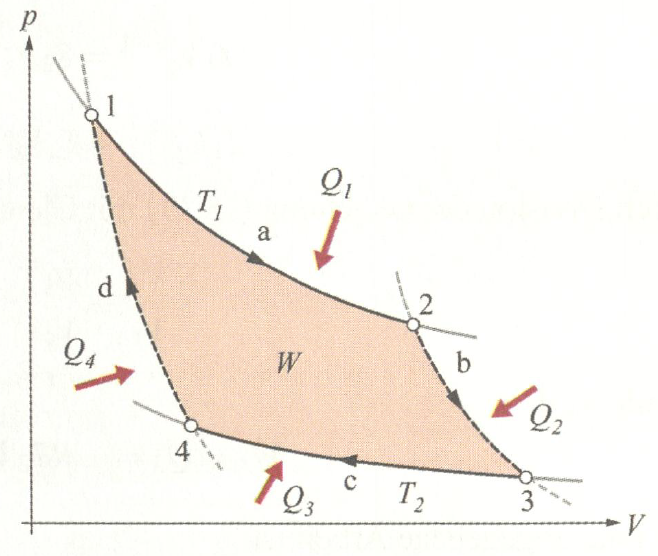
\includegraphics[width=7cm]{./bilder/KreisprozessCarnot.png}
			\end{minipage}
			\begin{minipage}[t]{10cm}
				\begin{enumerate}
					\vspace{1cm}
					\item isotheme Expansion bei der Temperatur $T_1$
					\item adiabatische Expansion
					\item isotherme Kompression bei der Temperatur $T_2$
					\item adiabatische Kompression
				\end{enumerate}
			\end{minipage}
		


%%%%%%%%%%%%%%%%%%%%%%%%%%%%%%%%%%%%%%%%%%%%%%%%%%%%%%%%%%%%%%%%%%%%%%%%%%%%%%%%%%%%%%%%%%%%%%%%
% Konstanten und griechische Buchstaben                                  
%%%%%%%%%%%%%%%%%%%%%%%%%%%%%%%%%%%%%%%%%%%%%%%%%%%%%%%%%%%%%%%%%%%%%%%%%%%%%%%%%%%%%%%%%%%%%%%%
\newpage
\section{Konstanten}
	\subsection{Dichte}
		\begin{tabular}{| p{6cm} | p{5cm} |}
			\hline
			\rowcolor{Gray}
			\textbf{Feststoffe}	&	$\boldsymbol{\rho}$ in $\dfrac{kg}{dm^3}$\\
			\hline
			Aluminium & $2.7$\\
			Blei & $11.34$\\
			Eis (0 \textdegree C) & 0.917\\
			Eisen & $6.6...7.4$\\
			Gold & $19.29$\\
			Holz trocken & $0.4...0.8$\\
			Kupfer & $8.9$\\
			& \\
			\hline
			\rowcolor{Gray}
			\textbf{Flüssigkeiten (@ 20 \textdegree C)} & $\boldsymbol{\rho}$ in $\dfrac{kg}{dm^3}$\\
			\hline
			Aceton & $0.79$\\
			Heizöl & $0.95...1.08$\\
			Wasser & $0.998$\\
			& \\
			\hline
			\rowcolor{Gray}
			\textbf{Gase (@ 0 \textdegree C und Normaldruck)}	&	$\boldsymbol{\rho}$ in $\dfrac{kg}{m^3}$\\
			\hline
			Helium & $0.178$\\
			Luft & $1.292$\\
			Sauerstoff & $1.428$\\
			Wasserstoff & $0.089$\\
			& \\
			\hline
		\end{tabular}
	
	\subsection{Spezifische Wärmekapazität}
		\begin{tabular}{| p{6cm} | p{5cm} |}
			\hline
			\rowcolor{Gray}
			\textbf{Feststoffe (@ 20 \textdegree C)}	&	$\boldsymbol{c}$ in $\dfrac{kJ}{kg \cdot K}$\\
			\hline
			Aluminium & $0.896$\\
			Blei & $0.129$\\
			Eis (0 \textdegree C) & $2.1$\\
			Eisen & $0.452$\\
			Gold & $0.129$\\
			Holz trocken & ca. $1.5$\\
			Kupfer & $0.382$\\
			& \\
			\hline
			\rowcolor{Gray}
			\textbf{Flüssigkeiten (@ 20 \textdegree C)} & $\boldsymbol{c}$ in $\dfrac{kJ}{kg \cdot K}$\\
			\hline
			Aceton & $2.16$\\
			Wasser & $4.182$\\
			& \\
			\hline
			\rowcolor{Gray}
			\textbf{Gase (@ 20 \textdegree C)}	&	$\boldsymbol{c}$ in $\dfrac{kJ}{kg \cdot K}$\\
			\hline
			Wasserdampf (@ 100 \textdegree C) & $1.87$\\
			Helium & $5.23$\\
			Luft & $1.005$\\
			Sauerstoff & $0.917$\\
			Wasserstoff & $14.32$\\
			& \\
			\hline
		\end{tabular}
	
	\subsection{Spezifische Schmelzwärme}
		\begin{tabular}{| p{6cm} | p{5cm} |}
			\hline
			\rowcolor{Gray}
			\textbf{Stoffe}	&	$\boldsymbol{q_f}$ in $\dfrac{kJ}{kg}$\\
			\hline
			Aluminium & $397$\\
			Blei & $23$\\
			Eisen & $277$\\
			Gold & $65.7$\\
			Kupfer & $205$\\
			Wasser & $334$\\
			& \\
			\hline
		\end{tabular}
	
	\subsection{Spezifische Verdampfungswärme}
		\begin{tabular}{| p{6cm} | p{5cm} |}
			\hline
			\rowcolor{Gray}
			\textbf{Stoffe (@ Normaldruck)}	&	$\boldsymbol{q_s}$ in $\dfrac{kJ}{kg}$\\
			\hline
			Aluminium & $10900$\\
			Blei & $8600$\\
			Eisen & $6339$\\
			Gold & $1650$\\
			Kupfer & $4790$\\
			Wasser & $2257$\\
			& \\
			\hline
		\end{tabular}
	
	\subsection{Kritische Temperatur}
		\begin{tabular}{| p{6cm} | p{5cm} |}
			\hline
			\rowcolor{Gray}
			\textbf{Stoffe}	&	$\boldsymbol{T_k}$ in $K$\\
			\hline
			Wasserstoff & $33.24$\\
			Helium & $5.2$\\
			Stickstoff & $126.2$\\
			Sauerstoff & $154.58$\\
			Wasser & $647.3$\\
			Methan & $19.56$\\
			Butan & 425.18\\
			Kohlendioxid & 304.3\\
			Gold & 7'850\\
			\hline
		\end{tabular}

\vspace{1cm}
\section{Griechsiche Buchstaben}
	\renewcommand{\arraystretch}{1.5}
	\begin{tabular}{| p{0.7cm} p{0.7cm} p{0.7cm} p{2cm} | p{0.7cm} p{0.7cm} p{0.7cm} p{2cm} | p{0.7cm} p{0.7cm} p{0.7cm} p{2cm} | }
		\hline
		A & $\alpha$ & & Alpha & I & $\iota$ & & Iota & P & $\varrho$ & $\rho$ & Rho\\
		B & $\beta$ & & Beta & K & $\varkappa$ & $\kappa$ & Kappa & $\Sigma$ & $\sigma$ & & Sigma\\
		$\Gamma$ & $\gamma$ & & Gamma & $\Lambda$ & $\lambda$ & & Lambda & T & $\tau$ & & Tau\\
		$\Delta$ & $\delta$ & & Delta & M & $\mu$ & & Mü & $\Upsilon$ & $\upsilon$ & & Ypsilon\\
		E & $\epsilon$ & & Epsilon & N & $\nu$ & & Nü & $\Phi$ & $\varphi$ & $\phi$ & Phi \\
		Z & $\zeta$ & & Zeta & $\Xi$ & $\xi$ & & Xi & X & $\chi$ & & Chi \\
		H & $\eta$ & & Eta & O & o & & Omikron & $\Psi$ & $\psi$ & & Psi\\
		$\Theta$ & $\vartheta$ & $\theta$ & Theta & $\Pi$ & $\pi$ & & Pi & $\Omega$ & $\omega$ & & Omega \\
		\hline
	\end{tabular}
	\renewcommand{\arraystretch}{1}	

%%%%%%%%%%%%%%%%%%%%%%%%%%%%%%%%%%%%%%%%%%%%%%%%%%%%%%%%%%%%%%%%%%%%%%%%%%%%%%%%%%%%%%%%%%%%%%%%
% Perieodensystem der Elemente                                   
%%%%%%%%%%%%%%%%%%%%%%%%%%%%%%%%%%%%%%%%%%%%%%%%%%%%%%%%%%%%%%%%%%%%%%%%%%%%%%%%%%%%%%%%%%%%%%%%
\newpage
\section{Periodensystem der Elemente}
	\begin{minipage}[t]{18cm}
		\begin{center}
			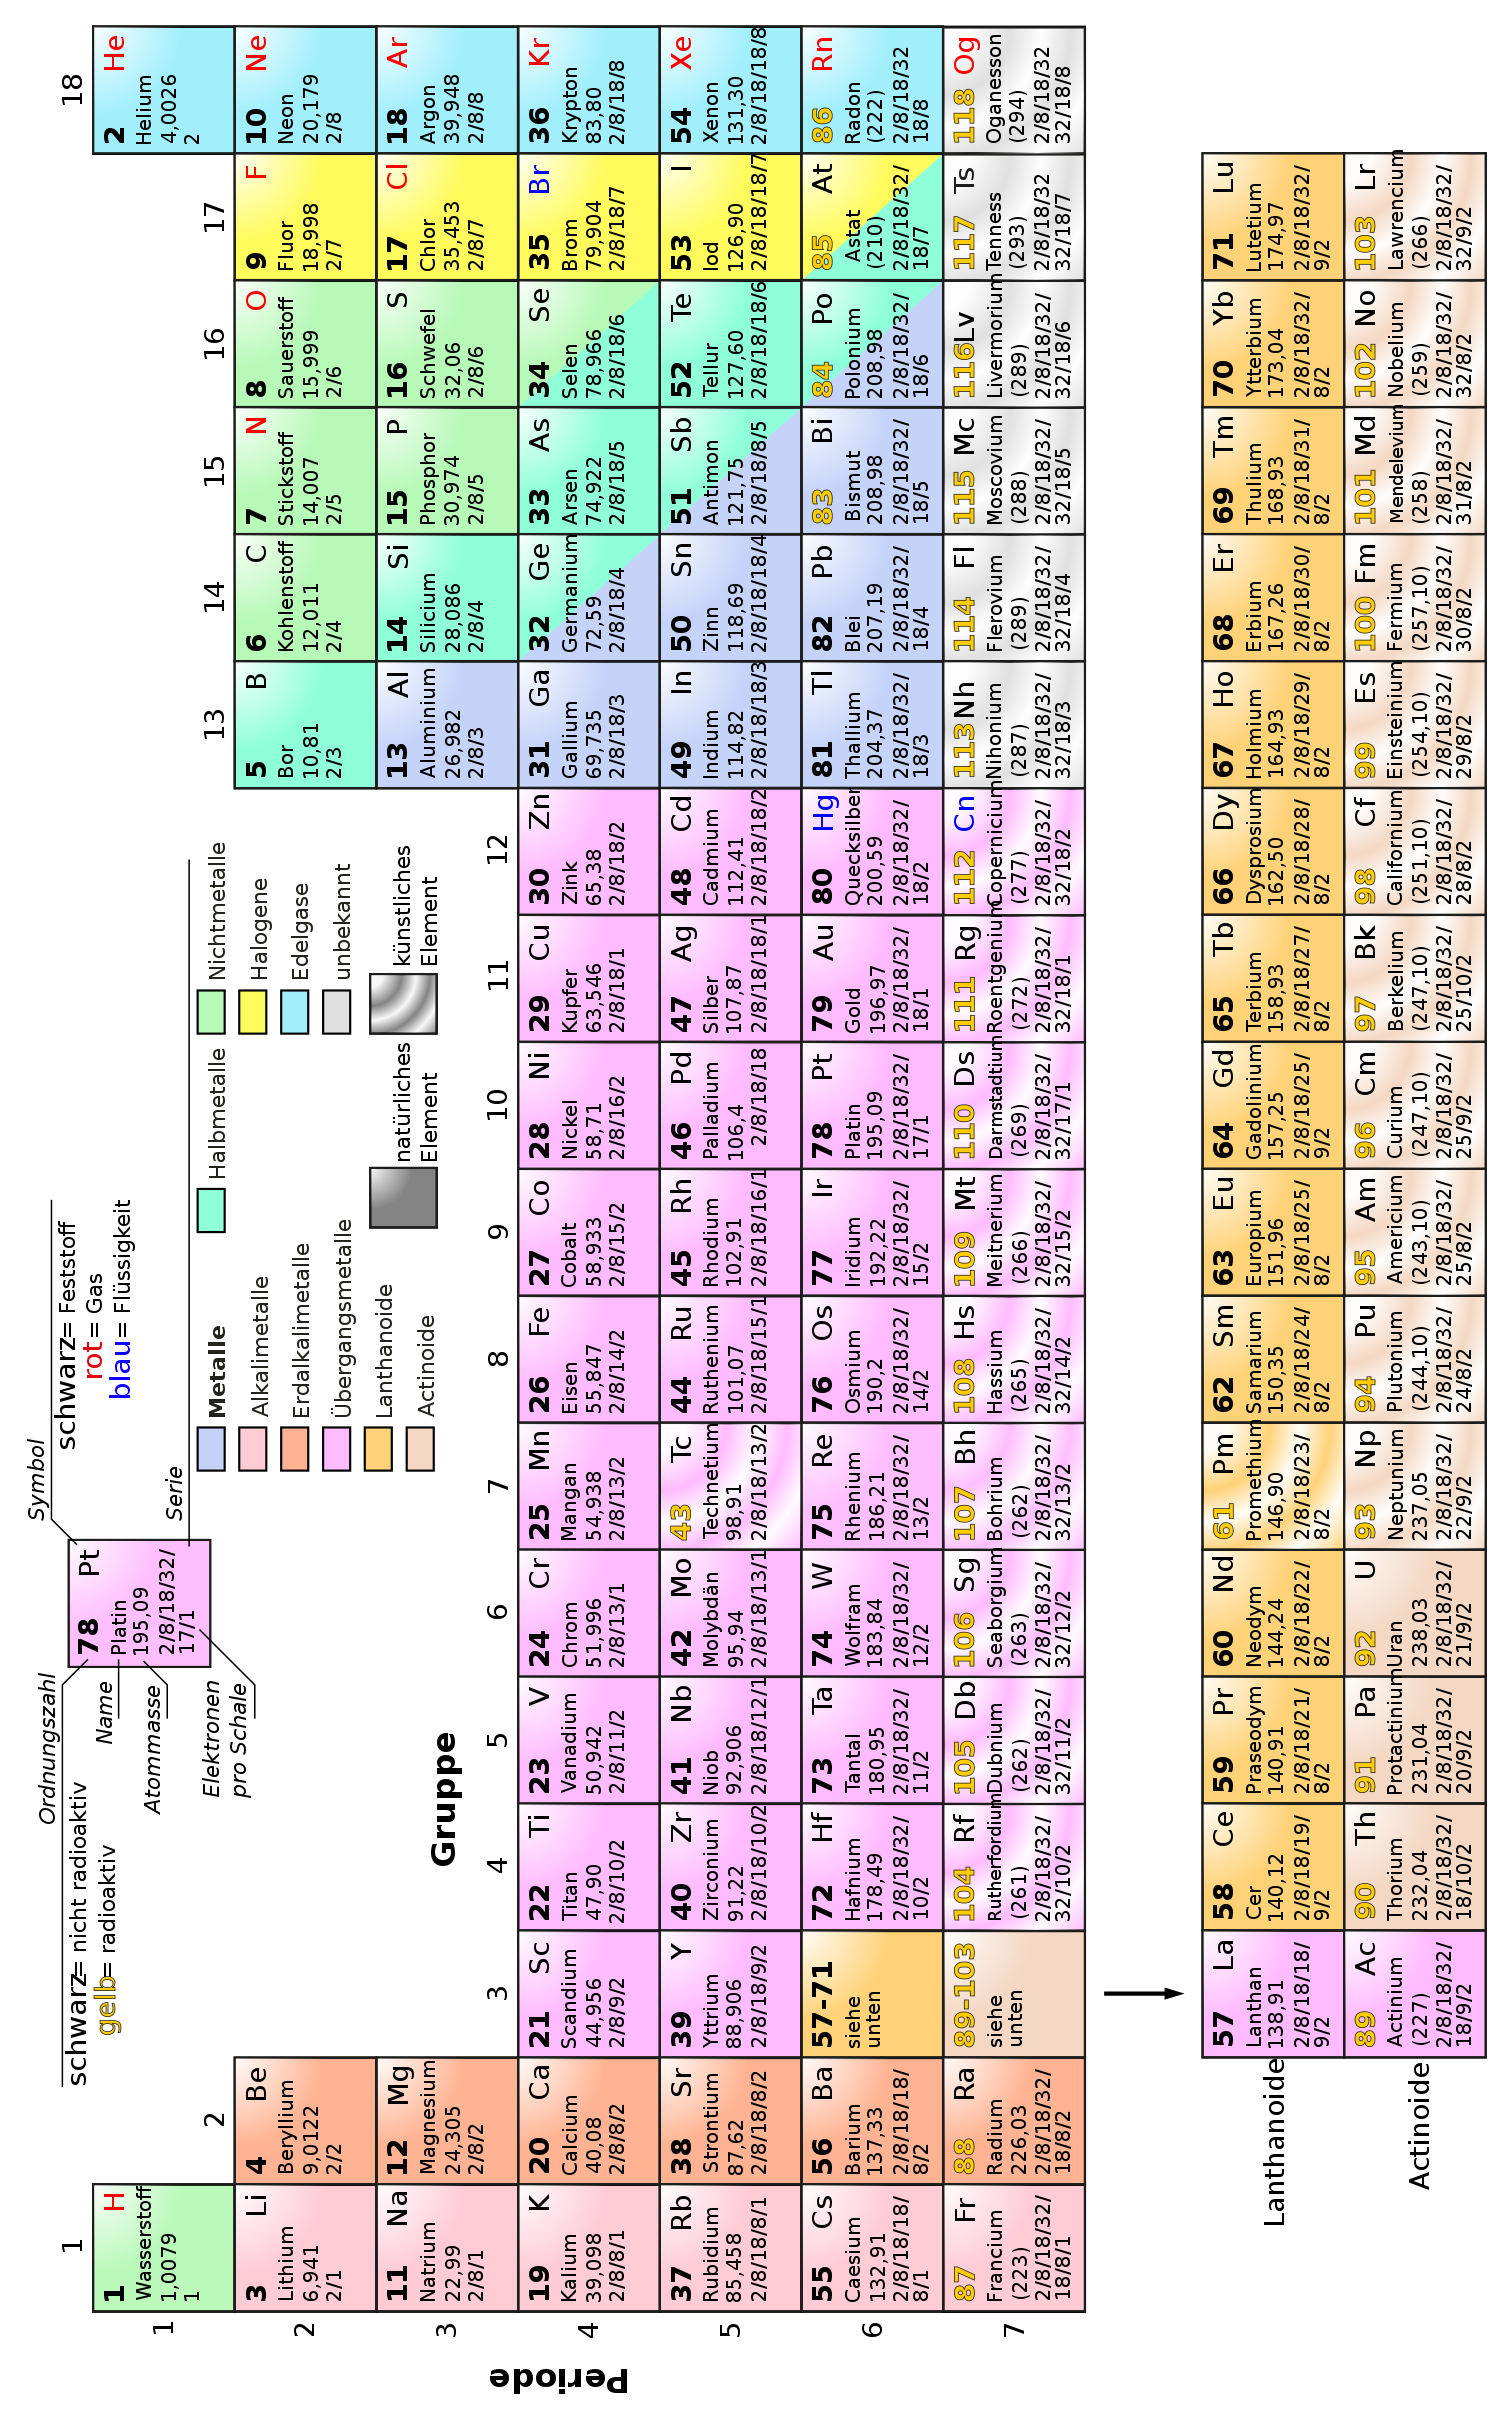
\includegraphics[width=15cm]{./bilder/Periodensystem.png}
			\newline
			Quelle: wikipedia.org [22. Juli 2019]
		\end{center}
	\end{minipage}
	

\end{document}